%!TEX root = main.tex

\documentclass[
  % draft,
  % final,
  a4paper,
  % 11pt,
  % twoside=semi,
  oneside,
  % parskip,
  toc=bibliography,
  toc=listof,
  chapterprefix=true,
]{scrbook}

%!TEX root = main.tex

%%% Grundlegendes

% Verwende etex als zugrundeliegende Implementierung (-> mehr Speicher für Tex!)
\usepackage{etex}
% Encoding
\usepackage[utf8]{inputenc}


%%% Schriften, Lokalisierung und Typographie

% T1 Schriftsystem verwenden
\usepackage[T1]{fontenc}
% LModern als Standard-Schrift
\usepackage{lmodern}
% Typographische Kleinigkeiten
\usepackage{microtype}
% Fraktur-Schriftsatz
\usepackage{eufrak}

%% Lokalisierung

% Deutsche Silbentrennung
\usepackage[english,ngerman]{babel}
% Deutsche Anführungszeichen
\usepackage[babel,german=quotes]{csquotes}

%% Weitere Schriften vordefinieren

\newcommand{\altfont}{\fontfamily{qpl}}
% \newcommand{\altsffont}{\fontfamily{phv}}
\newcommand{\altsffont}{\fontfamily{pfr}\fontseries{l}}

% Zeilenabstand anpassen (MUST NOT USE!)
% \usepackage{setspace}
% \setstretch{1.1}

% Textsatzbereich nach unten vergrößern
% TODO: richtig konfigurieren
% \usepackage[a4paper,twoside,bottom=4cm]{geometry}

%%% Graphiken und Farben

% Graphiken und Farben
\usepackage{xcolor}
\usepackage{graphicx}

% Vordefinierte Farben laden
\definecolor{jgu_rot}{RGB}{193,0,42}
\definecolor{jgu_hellgrau}{RGB}{172,172,172}
\definecolor{jgu_dunkelgrau}{RGB}{99,99,99}
\definecolor{matlab_blau}{rgb}{0.00000,0.44700,0.74100}
\definecolor{matlab_orange}{rgb}{0.85000,0.32500,0.09800}


% Caption anpassen und Subfigures erlauben
\usepackage[style=base,font+=small,labelfont+=bf,margin=1em]{caption}
\usepackage{subcaption}

% Tikz ist kein Zeichenprogramm!
\usepackage{tikz}
\usepackage{pgfplots}
\pgfplotsset{compat=1.12}
\usetikzlibrary{patterns}

% Standalone-Paket, damit die Tikz Bilder extern auch funktionieren
\usepackage{standalone}


%%% Bibliographie

\usepackage[%
    backend=biber,
    style=alphabetic,
    backref=true,
    firstinits=true
]{biblatex}

% Fix für doi2bib generierte Bibliography-Einträge
\newcommand\mathplus{+}


%%% Grundlegende Mathematik-Pakete

% Standardpackages
\usepackage{amsmath}
\usepackage{amssymb}
\usepackage{stmaryrd}
\usepackage{mathtools}

% "Bessere" Theorem-Umgebungen
\usepackage[
    amsmath,
    thmmarks,
    hyperref,
]{ntheorem}


%%% Hyperref

\usepackage[
	colorlinks=true,
	linkcolor=jgu_rot,          % color of internal links (change box color with linkbordercolor)
	citecolor=jgu_rot,        % color of links to bibliography
	filecolor=jgu_rot,      % color of file links
	urlcolor=jgu_rot,
    hypertexnames=false
]{hyperref}


%%% Clevere Referenzen

\usepackage[german,noabbrev,nameinlink,capitalise]{cleveref}
\crefname{equation}{}{}

% Nummern nur für referenzierte Gleichungen
\usepackage{autonum}


%%% Layout und Stil

% Fancyhdr-Ersatz für scrbook
\usepackage[
    automark,
    % headsepline,
    draft=false
]{scrlayer-scrpage}

% Inhaltsverzeichnis anpassen (Schriften angleichen!)
\usepackage{tocstyle}
\usetocstyle{KOMAlike}

%% Chapter-Style und mehr

% Alle Überschriften in TeX Gyre Pagella
\addtokomafont{disposition}{\normalfont\altfont\selectfont}
% Alle Überschriften in Dunkelgrau
% \addtokomafont{disposition}{\color{jgu_dunkelgrau}}

% Einzelne Optionen bei Bedarf
% \addtokomafont{chapter}{\normalfont\altfont\selectfont}
% \addtokomafont{chapter}{\color{black}}
% \addtokomafont{section}{\normalfont\altfont\selectfont}
% \addtokomafont{subsection}{\normalfont\altfont\selectfont}
% \addtokomafont{subsubsection}{\normalfont\altfont\selectfont}
% \addtokomafont{minisec}{\normalfont\altfont\selectfont}
% \addtokomafont{paragraph}{\normalfont\altfont\selectfont}
\addtokomafont{paragraph}{\bfseries}

% Kopfzeile anpassen
\addtokomafont{pageheadfoot}{\color{jgu_dunkelgrau}\normalfont\altfont\selectfont}
% Seitenzahl anpassen
\addtokomafont{pagenumber}{\color{jgu_dunkelgrau}\normalfont\altfont\selectfont}

% Zitatblock für Kapitelanfang
\renewcommand*\dictumwidth{.95\linewidth}
\renewcommand*\dictumrule{}
\renewcommand*\dictumauthorformat[1]{--- #1}
\addtokomafont{dictumtext}{\color{jgu_dunkelgrau}\normalfont\altsffont\fontsize{9}{12}\selectfont\itshape}
\addtokomafont{dictumauthor}{\color{jgu_dunkelgrau}\normalfont\altsffont\fontsize{8}{12}\selectfont}

% Kapitel-Stil
\renewcommand*{\chapterheadstartvskip}{\vspace*{3\baselineskip}}
\renewcommand*{\chapterheadendvskip}{\vspace*{2\baselineskip}}
\renewcommand*{\chapterformat}{%
				\raggedright
				\color{jgu_rot}
                \altfont\fontsize{60}{30}\selectfont\thechapter
                \fontsize{20}{30}\scshape\selectfont\enskip\chapappifchapterprefix
                }
\renewcommand*{\raggedchapter}{\raggedleft}

% Inhaltsverzeichnis
% \addtokomafont{sectionentrypagenumber}{\color{black}}
\addtokomafont{chapterentrypagenumber}{\color{black}\rmfamily}
\addtokomafont{chapterentry}{\rmfamily\bfseries}


%%% Verzeichnisse

% Akronymverzeichnis
\usepackage{acro}
\acsetup{
    page-ref=paren,
    pages=first,
    page-name={siehe S.\@\,},
}

% Symbolverzeichnis
\usepackage[german,intoc]{nomencl}
\setlength{\nomitemsep}{-\parsep}
\makenomenclature


% ntheorem-Umgebungen laden
%%
%% This is file `ntheorem.std',
%% generated with the docstrip utility.
%%
%% The original source files were:
%%
%% ntheorem.dtx  (with options: `standard')
%%
%% IMPORTANT NOTICE:
%%
%% For the copyright see the source file.
%%
%% Any modified versions of this file must be renamed
%% with new filenames distinct from ntheorem.std.
%%
%% For distribution of the original source see the terms
%% for copying and modification in the file ntheorem.dtx.
%%
%% This generated file may be distributed as long as the
%% original source files, as listed above, are part of the
%% same distribution. (The sources need not necessarily be
%% in the same archive or directory.)
\def\filedate{2011/08/15}
\def\docdate{2011/08/15}
\def\fileversion{1.33}
\def\basename{ntheorem}
%% This file may be distributed and/or modified under the
%% conditions of the LaTeX Project Public License, either version 1.2
%% of this license or (at your option) any later version.
%% The latest version of this license is in
%%    http://www.latex-project.org/lppl.txt
%% and version 1.2 or later is part of all distributions of LaTeX
%% version 1999/12/01 or later.
%% \CharacterTable
%%  {Upper-case    \A\B\C\D\E\F\G\H\I\J\K\L\M\N\O\P\Q\R\S\T\U\V\W\X\Y\Z
%%   Lower-case    \a\b\c\d\e\f\g\h\i\j\k\l\m\n\o\p\q\r\s\t\u\v\w\x\y\z
%%   Digits        \0\1\2\3\4\5\6\7\8\9
%%   Exclamation   \!     Double quote  \"     Hash (number) \#
%%   Dollar        \$     Percent       \%     Ampersand     \&
%%   Acute accent  \'     Left paren    \(     Right paren   \)
%%   Asterisk      \*     Plus          \+     Comma         \,
%%   Minus         \-     Point         \.     Solidus       \/
%%   Colon         \:     Semicolon     \;     Less than     \<
%%   Equals        \=     Greater than  \>     Question mark \?
%%   Commercial at \@     Left bracket  \[     Backslash     \\
%%   Right bracket \]     Circumflex    \^     Underscore    \_
%%   Grave accent  \`     Left brace    \{     Vertical bar  \|
%%   Right brace   \}     Tilde         \~}

\theoremnumbering{arabic}
\theoremstyle{plain}
\RequirePackage{latexsym}
% \theoremsymbol{\ensuremath{_\Box}}
\theorembodyfont{\itshape}
\theoremheaderfont{\normalfont\bfseries}
\theoremseparator{}
\newtheorem{Theorem}{Theorem}[chapter]
\newtheorem{theorem}[Theorem]{Theorem}
\newtheorem{Satz}[Theorem]{Satz}
\newtheorem{satz}[Theorem]{Satz}
\newtheorem{Proposition}[Theorem]{Proposition}
\newtheorem{proposition}[Theorem]{Proposition}
\newtheorem{Lemma}[Theorem]{Lemma}
\newtheorem{lemma}[Theorem]{Lemma}
\newtheorem{Korollar}[Theorem]{Korollar}
\newtheorem{korollar}[Theorem]{Korollar}
\newtheorem{Corollary}[Theorem]{Corollary}
\newtheorem{corollary}[Theorem]{Corollary}

\theorembodyfont{\upshape}
\newtheorem{Example}[Theorem]{Example}
\newtheorem{example}[Theorem]{Example}
\newtheorem{Beispiel}[Theorem]{Beispiel}
\newtheorem{beispiel}[Theorem]{Beispiel}
\newtheorem{Bemerkung}[Theorem]{Bemerkung}
\newtheorem{bemerkung}[Theorem]{Bemerkung}
\newtheorem{Anmerkung}[Theorem]{Anmerkung}
\newtheorem{anmerkung}[Theorem]{Anmerkung}
\newtheorem{Remark}[Theorem]{Remark}
\newtheorem{remark}[Theorem]{Remark}
\newtheorem{Definition}[Theorem]{Definition}
\newtheorem{definition}[Theorem]{Definition}
\newtheorem{Annahme}[Theorem]{Annahme}
\newtheorem{annahme}[Theorem]{Annahme}

\theoremstyle{nonumberplain}
\theoremheaderfont{\scshape}
\theorembodyfont{\normalfont}
\theoremseparator{.}
\theoremsymbol{\ensuremath{_\square}}
\RequirePackage{amssymb}
\newtheorem{Proof}{Proof}
\newtheorem{proof}{Proof}
\newtheorem{Beweis}{Beweis}
\newtheorem{beweis}{Beweis}
\qedsymbol{\ensuremath{_\square}}

\theoremstyle{nonumberplain}
\theoremheaderfont{\normalfont\bfseries}
\theoremseparator{}
\theorembodyfont{\normalfont}
\theoremsymbol{}
\RequirePackage{amssymb}
\newtheorem{Problem}{Problem}
\newtheorem{problem}{Problem}
\qedsymbol{}

\theoremclass{LaTeX}
\endinput
%%
%% End of file `ntheorem.std'.



%%% Alles andere

% Querformatseiten
\usepackage{pdflscape}

% Enumerates anpassen
\usepackage{enumitem}
% Numerierte Umgebung für Theoreme definieren
\newlist{thmenumerate}{enumerate}{1}
\setlist[thmenumerate]{label={\upshape(\roman*)}, align=left, widest=iii, leftmargin=*}
\crefname{thmenumeratei}{}{}

% Konturen um Text zeichnen
\usepackage[outline]{contour}
\contourlength{0.09em}

% Gepunktete Linien
\usepackage{dashrule}


%%% "Debugging"

% Labels am Seitenrand anzeigen
\usepackage[
    inline,
    final
]{showlabels}

% todos
\usepackage[%
    german,
    colorinlistoftodos,
    % disable
]{todonotes}

% Todos vordefinieren
\newcommand{\mdo}[1]{\todo[color=yellow!50]{#1}}
\newcommand{\mfix}[1]{\todo[color=red!50]{#1}}
\newcommand{\mwarn}[1]{\todo[color=blue!50]{#1}}

% Blindtext
\usepackage{blindtext}
\blindmathtrue{}

% etoolbox?
\usepackage{etoolbox}

% \usepackage{showframe}



%!TEX root = main.tex

% griechisches Alphabet anpassen
\renewcommand{\epsilon}{\varepsilon}
\renewcommand{\theta}{\vartheta}


%%% Operatoren und anderes mathematisches Geplänkel

% Beträge und Normen
\DeclarePairedDelimiter{\abs}{\lvert}{\rvert}
\DeclarePairedDelimiter{\norm}{\lVert}{\rVert}

% Gauß-Klammern
\DeclarePairedDelimiter{\ceil}{\lceil}{\rceil}
\DeclarePairedDelimiter{\floor}{\lfloor}{\rfloor}

% Skalarprodukte und Duale Paarungen
\newcommand{\skprod}[2]{\left\langle#1,#2\right\rangle}
\newcommand{\Skp}[3]{\left\langle#1,#2\right\rangle_{#3}}
\newcommand{\skp}[3]{\langle#1,#2\rangle_{#3}}
\newcommand{\Dual}[2]{\left(#1,#2\right)}
\newcommand{\dual}[2]{(#1,#2)}

% Inneres und Äußeres
\newcommand{\Int}[1]{#1^\circ}
\newcommand{\Ext}[1]{\overline{#1}}

% Diverse Operatoren
\DeclareMathOperator{\spn}{span}
\DeclareMathOperator{\ee}{e}
\DeclareMathOperator{\ii}{i}
\newcommand{\Transp}{^{\mathrm{T}}}
\newcommand{\Stern}{^{*}}
\newcommand{\grad}{\nabla}
\DeclareMathOperator{\divergenz}{div}
\newcommand{\hesse}{\nabla^2}

% Einschränkung einer Funktion
\newcommand\restr[2]{\ensuremath{\left.#1\right|_{#2}}}

% Ordentlicher Befehl um Mengen zu setzen
\providecommand\given{} % so it exists
\newcommand\SetSymbol[1][]{
   \nonscript\,#1\vert\nonscript\,\mathopen{}\allowbreak}
\DeclarePairedDelimiterX\Set[1]{\lbrace}{\rbrace}{ \renewcommand\given{\SetSymbol[\delimsize]} #1 }

% Vektoren und Matrizen anders setzen
\renewcommand{\vec}[1]{\mathbf{#1}}
\newcommand{\mat}[1]{\mathbf{#1}}

% Differential-d für Integral ordentlich setzen
\newcommand*\diff{\mathop{}\!\mathrm{d}}
\newcommand*\Diff[1]{\mathop{}\!\mathrm{d^#1}}

% wesentliches Supremum
\DeclareMathOperator*{\esssup}{ess\,sup}
\newcommand\blank{{\mkern2mu\cdot\mkern2mu}}

% "Definition-Gleich"
% FIXME: deprecated
\newcommand\deq{\coloneqq}

% dichte Einbettung
% FIXME: zu hoch für Fließtext!
\newcommand\denseinclusion{\stackrel{d}{\hookrightarrow}}

% Schrift einfach anpassen
\newcommand{\changefont}[3]{
\fontfamily{#1} \fontseries{#2} \fontshape{#3} \selectfont}


%%% Textbausteine

\newcommand{\fa}{\text{für alle}~}

% um fremde Begriffe einheitlich mit Übersetzung zu setzen
\newcommand\foreign[2]{#1 \textit{#2}}

%!TEX root = main.tex

\newcommand{\titel}{- in Arbeit - Parabolische partielle Differentialgleichungen und Reduzierte-Basis-Methoden}
\newcommand{\art}{Masterarbeit}
\newcommand{\autor}{Alexej Disterhoft}
\newcommand{\fach}{Mathematik}
\newcommand{\matrikelnr}{2669611}
\newcommand{\erstgutachter}{JProf. Dr. Thorsten Raasch}
\newcommand{\zweitgutachter}{???}
\newcommand{\monat}{Irgendwann}
\newcommand{\jahr}{2015}
\newcommand{\ort}{Mainz}
\newcommand{\logo}{figures/misc/logo_gross.eps}

\hypersetup{pdfinfo={
  Title=\titel,
  Author=\autor}
}


\begin{document}

    % Deckblack / Titelseite
    %!TEX root = ../main.tex

\thispagestyle{plain}
\begin{titlepage}
\begin{center}
% $\;$\\[2em]
\includegraphics[scale=1.5,clip,trim=0em 2em 0em 2.8em]{\logo}\\[3em]
%
% {\fontfamily{qpl}\selectfont{\LARGE{\textbf{\titel}}\par}}
{\fontfamily{qpl}\selectfont{\LARGE{\textbf{Numerische Behandlung von \\Self-Consistent Field Theory-Modellen\\ mittels Reduzierter-Basis-Methoden}}\par}}
\normalsize$\;$\\[1em]
{\large{\textbf{\art}}}\\[1em]
{\normalsize
am Institut für Mathematik,\\
Fachbereich Physik, Mathematik und Informatik\\
der Johannes Gutenberg-Universität\\
in Mainz
}\\[6em]
%
{\large{\textbf{\autor}}}\\[0.4em]
{\normalsize{geboren in Leonidowka}}\\[4em]
%
\begin{tabular}{p{3cm}p{7cm}}\\
Erstgutachter:  & \quad \erstgutachter\\[1.2ex]
Zweitgutachter: & \quad \zweitgutachter\\[3ex]
\end{tabular}

{\ort,~\today}
% {\ort,~\monat~\jahr}
%
\end{center}
\end{titlepage}


    %%%%%%%%%%%%%%%%%%%%%%%%%%%%%%%%%%%%%%%%%%%%%%%%%%%%%%%%%%%%%%%%%%%%%%%%%%%
    %%% Frontmatter-Teil
    \frontmatter{}

    % Danksagung
    % %!TEX root = ../main.tex

\thispagestyle{plain}
\begin{titlepage}
\dictum[Andy Weir, \textit{The Martian}]{\enquote{I guess you could call it a \enquote{failure}, but I prefer the term \enquote{learning
experience}.}}
\vfill{}
\begin{flushright}
% \emph{Für meine Eltern.}
\end{flushright}
\end{titlepage}


    % Abstrakt
    % %!TEX root = ../main.tex

\chapter{Zusammenfassung} % (fold)
\label{cha:Zusammenfassung}

\blindtext

% chapter Zusammenfassung (end)


    % Inhaltsverzeichnis
    \tableofcontents

    % TODO-Liste
    % \listoftodos

    %%%%%%%%%%%%%%%%%%%%%%%%%%%%%%%%%%%%%%%%%%%%%%%%%%%%%%%%%%%%%%%%%%%%%%%%%%%
    %%% Hauptteil
    \mainmatter{}

    % Kapitel
    % %!TEX root = ../main.tex

\chapter{Einleitung} % (fold)
\label{cha:einleitung}

\blindmathpaper

% chapter einleitung (end)

    %!TEX root = ../main.tex

\chapter{Grundlagen} % (fold)
\label{cha:grundlagen}

Verschiedenste Grundlagen, die hier abgedeckt werden sollten.
Dazu gehören folgende Abschnitte:

\section{Funktionalanalytische Grundlagen} % (fold)
\label{sec:funktionalanalytische_grundlagen}

\subsection{Bochner-Räume} % (fold)
\label{sub:bochner_r_ume}

\begin{Definition}[Bochner-Räume]
    Sei $X$ ein Banachraum, $(a, b) \subset \mathbb{R}$, $- \infty \leq a < b \leq \infty$, ein offenes Intervall und $1 \leq p < \infty$.
    Wir nennen $L_{p}(a, b; X)$ einen Bochner-Raum und meinen damit die Menge der Äquivalenzklassen $L_{p}$-integrierbarer Funktionen $f \colon [a, b] \to X$, das heißt alle Lebesgue-messbaren Funktionen auf $[a, b]$ mit
    \begin{equation}
        \norm{f}_{L_{p}(a, b; X)} \coloneqq \left( \int_{a}^{b} \norm{f(t)}_{X}^{p} \diff t \right)^{\frac 1 p} < \infty.
    \end{equation}
    Analog bezeichnen wir mit $L_{\infty}(a, b; X)$ die Menge der Äquivalenzklassen die fast überall auf $[a, b]$ beschränkt sind, das heißt
    \begin{equation}
        \norm{f}_{L_{\infty}(a, b; X)} \coloneqq \esssup_{t \in [a, b]} \norm{f(t)}_{X} < \infty.
    \end{equation}
\end{Definition}

\begin{Lemma}
    Sei $1 \leq p \leq \infty$. Dann ist $L_{p}(a, b; X)$ ein Banachraum.
    Ist $H$ ein Hilbertraum, dann ist insbesondere auch $L_{2}(a, b; H)$ ein Hilbertraum.
\end{Lemma}

\begin{Lemma}[Eigenschaften]
    \begin{enumerate}
        \item Ist $[a, b] \subset \mathbb{R}$ ein endliches Intervall, dann gilt die stetige Einbettung
        \begin{equation}
            L_{q}(a, b; X) \hookrightarrow L_{p}(a, b; X), \qquad q \geq p \geq 1.
        \end{equation}
        \item Sind $X$ und $Y$ Banachräume mit $X \hookrightarrow Y$, dann gilt die stetige Einbettung
        \begin{equation}
            L_{p}(a, b; X) \hookrightarrow L_{p}(a, b; Y), \qquad 1 \leq p \leq q.
        \end{equation}
    \end{enumerate}
\end{Lemma}

    %!TEX root = ../main.tex

\chapter{Parametrisches Problem} % (fold)
\label{cha:parametrisches_problem}

% TODO: Anpassen an Zeitabhängige lineare Operatoren bzw. Bilinearformen!

In diesem Kapitel liegt das Augenmerk erneut auf der linearen Evolutionsgleichung \eqref{eq:allgemeine_parabolische_pde}, diesmal aber mit der Erweiterung, dass der lineare Operator $A(t)$ zusätzlich von einem Parameter $\sigma$ abhängt.

Zunächst konkretisieren wir diese Parameterabhängigkeit für einen linearen Operator $A$, betrachten dann eine parametrische lineare Operatorgleichung, leiten Regularitätsergebnisse für diese her und übertragen diese anschließend auf die Raum-Zeit-Variationsformulierung einer parametrischen linearen Evolutionsgleichung.
Dabei orientieren wir uns hauptsächlich an den Arbeiten von \textcite{Kunoth:2013ef,Cohen:2010kz}.

\section{Parametrische Operatorgleichung} % (fold)
\label{sec:parametrische_operatorgleichung}

Seien $X$ und $Y$ zwei reflexive Banachräume.
Weiter sei $\mathcal S \subset \mathbb{R}^{\mathbb{N}}$ der sogenannte Parameterraum.
Der Einfachheit halber wählen wir $\mathcal S = [-1, 1]^{\mathbb{N}}$. % TODO: warum?

Wir betrachten parametrische Familien stetiger linearer Operatoren $A(\sigma) \in \mathcal L(X, Y')$ mit $\sigma \in \mathcal S$.
Folgende lineare Operatorgleichung ist für uns von Interesse:
Sei ein $g \in Y'$ gegeben.
Finde für alle $\sigma \in \mathcal S$ eine Lösung $u(\sigma) \in X$ von
\begin{equation}
    \label{eq:allgemeine_parametrische_elliptische_pde}
    A(\sigma) u(\sigma) = g \quad \text{in}~Y'.
\end{equation}
Wie zuvor sei $a(\blank, \blank; \sigma) \colon X \times Y \to \mathbb{R}$ die zugehörige Bilinearform.

Zunächst einige notationelle Vorbemerkungen.
\begin{Bemerkung}
    Wir bezeichnen mit $\mathfrak F = \Set{ \nu \in \mathbb{N}^{\mathbb{N}}_{0} \given \abs{\nu} < \infty }$ die Menge aller Folgen nichtnegativer ganzer Zahlen mit endlichem Träger, das heißt nur endlich vielen Einträgen ungleich Null.
    % NOTE: Eventuell mehr definieren, siehe $\mathfrak n$ und $\mathfrak m$

    Sei $\nu \in \mathfrak F$ und $b \in \ell_{p}(\mathbb{N})$, $p > 0$, dann schreiben wir
    \begin{equation}
        b^{\nu} = \prod_{j = 1}^{\infty} b_{j}^{\nu_{j}}
    \end{equation}
    mit der Konvention $0^{0} = 1$.
    Wegen $\abs{\nu} < \infty$ ist dieses Produkt stets endlich.
\end{Bemerkung}

Für die nachfolgenden Regularitätsaussagen über die Lösung $u(\sigma)$ von \eqref{eq:allgemeine_parametrische_elliptische_pde} benötigen wir Regularität der Operatorfamilie $A(\sigma)$ bezüglich $\sigma \in \mathcal S$.
Konkret fordern wir:
\begin{Annahme}[{{\cite[Assumption 1]{Kunoth:2013ef}}}]
\label{thm:kunoth:assumption1}
    Die parametrische Familie von Operatoren
    $\Set{ A(\sigma) \in \mathcal L(X, Y') \given \sigma \in \mathcal S }$ sei eine $\mathfrak p$-reguläre Operatorfamilie für ein $0 < \mathfrak p \leq 1$, das heißt,
    \begin{thmenumerate}
        \item $A(\sigma) \in \mathcal L(X, Y')$ sei stetig invertierbar für alle $\sigma \in \mathcal S$ mit gleichmäßig beschränktem Inversen $A{(\sigma)}^{-1} \in \mathcal L(Y', X)$, das heißt, es existiert ein $C_{0} > 0$ mit
        \begin{equation}
            \sup_{\sigma \in \mathcal S} \norm{A{(\sigma)}^{-1}}_{\mathcal L(Y', X)} \leq C_{0},
        \end{equation}
        \item für jedes feste $\sigma \in \mathcal S$ seien die Operatoren $A(\sigma)$ analytisch bezüglich $\sigma$.
        Konkret existiert eine nichtnegative Folge $b = (b_{j})_{j \in \mathbb{N}} \in \ell_{\mathfrak p}(\mathbb{N})$, so dass
        \begin{equation}
            \sup_{\sigma \in \mathcal S} \norm{(A{(0)})^{-1}(\partial^{\nu}_{\sigma} A(\sigma))}_{\mathcal L(X, X)} \leq C_{0} b^{\nu}
        \end{equation}
        für alle $\nu \in \mathfrak F \setminus \{ 0 \}$ gilt.
        Dabei sei $\partial^{\nu}_{\sigma} A(\sigma) \deq \frac{\partial^{\nu_{1}}}{\partial \sigma_{1}} \frac{\partial^{\nu_{2}}}{\partial \sigma_{2}} \cdots A(\sigma)$.
    \end{thmenumerate}
\end{Annahme}

Die bisherigen Anforderungen an $A(\sigma)$ decken einen noch sehr weiten Bereich ab.
Wir beschränken uns in dieser Arbeit ausschließlich auf den folgenden Fall, der affin parametrischen Operatoren.

\begin{Definition}
    Sei $\Set{ A(\sigma) \in \mathcal L(X, Y') \given \sigma \in \cal S }$ eine parametrische Operatorfamilie.
    Wir nennen $A(\sigma)$ einen \emph{affin parametrischen Operator}, falls eine Familie von Operatoren $\Set{ \hat A, A_{j} \given j \in \mathbb{N} } \subset \cal L(X, Y')$ existiert, so dass
    \begin{equation}
        \label{eq:all_affiner_operator}
        A(\sigma) = \hat A + \sum_{j = 1}^{\infty} \sigma_{j} A_{j} \qquad\fa \sigma \in \mathcal S
    \end{equation}
    gilt.
\end{Definition}

Seien $\hat a, a_{j} \colon X \times Y \to \mathbb{R}$ die durch den Rieszschen Darstellungssatz von $\hat A$ respektive $A_{j}$ induzierten Bilinearformen, das heißt also,
\begin{equation}
    \label{eq:allg_affine_bf}
    \begin{aligned}
    \hat a(\eta, \zeta) &= \skprod{\hat A \eta}{\zeta}_{Y' \times Y}
    \\
    a_{j}(\eta, \zeta) &= \skprod{A_{j} \eta}{\zeta}_{Y' \times Y}, \quad j \in \mathbb{N},
    \end{aligned}
\end{equation}
für $\eta \in X$, $\zeta \in Y$.

Um die Wohldefiniertheit von $A(\sigma)$, das heißt Konvergenz von \eqref{eq:all_affiner_operator}, sicherzustellen, stellen wir folgende Bedingungen:
\begin{Annahme}[{{\cite[Assumption 2]{Kunoth:2013ef}}}]
\label{thm:kunoth:assumption2}
    Die Operatorfamilie $\Set{\hat A, A_{j} \given j \in \mathbb{N}}$ erfülle folgende Eigenschaften:
    \begin{thmenumerate}
        \item Der \emph{Mean Field}-Operator $\hat A \in \mathcal L(X, Y')$ sei stetig invertierbar, das heißt, es existiert ein $\gamma_{0} > 0$ mit
        \begin{subequations}\label{eq:kunoth:ass2_gamma_0}
            \begin{align}
                \label{eq:kunoth:ass2_gamma_0_a}
                \inf_{0 \neq u \in X} \sup_{0 \neq v \in Y} \frac{\hat a(u, v)}{\norm{u}_{X} \norm{v}_{Y}} \geq \gamma_{0}
                \intertext{und}
                \label{eq:kunoth:ass2_gamma_0_b}
                \inf_{0 \neq v \in Y} \sup_{0 \neq u \in X} \frac{\hat a(u, v)}{\norm{u}_{X} \norm{v}_{Y}} \geq \gamma_{0}.
            \end{align}
        \end{subequations}
        \item Die \emph{Fluctuation}-Operatoren $\Set{ A_{j} }_{j \geq 1}$ seien \emph{klein} relativ zu $\hat A$ im folgenden Sinne: es existiert eine Konstante $0 < \kappa < 1$ so dass
        \begin{equation}
            \label{eq:kunoth:ass2_abs_reihe}
            \sum_{j = 1}^{\infty} \norm{A_{j}}_{\mathcal L(X, Y')} \leq \kappa \gamma_{0}
        \end{equation}
        gilt.
    \end{thmenumerate}
\end{Annahme}

Unter diesen Bedingungen liefert das Banach-Ne{\v c}as-Babu{\v s}ka-Theorem, \thref{satz:gl:bnb_theorem}, die stetige Invertierbarkeit von $A(\sigma)$ aus \eqref{eq:all_affiner_operator} gleichmäßig in $\sigma$.

\begin{Satz}[{{\cite[Theorem 2]{Kunoth:2013ef}}}]
    Der affin parametrische Operator $A(\sigma)$ erfülle \thref{thm:kunoth:assumption2}.
    Dann ist $A(\sigma)$ für alle $\sigma \in \mathcal S$ stetig invertierbar.

    Konkret gilt
    \begin{equation}
        \inf_{u \in H_{1}} \sup_{v \in H_{2}} \frac{a(u, v)}{\norm{u}_{H_{1}} \norm{v}_{H_{2}}} \geq (1 - \kappa) \gamma_{0} > 0 \quad \fa \sigma \in \mathcal S
    \end{equation}
    und
    \begin{equation}
        \inf_{v \in H_{2}} \sup_{u \in H_{1}} \frac{a(u, v)}{\norm{u}_{H_{1}} \norm{v}_{H_{2}}} \geq (1 - \kappa) \gamma_{0} > 0 \quad \fa \sigma \in \mathcal S.
    \end{equation}

    Ist ferner ein $g \in Y'$ gegeben, dann existiert für jedes $\sigma \in \mathcal S$ ein $\hat u(\sigma) \in X$ mit
    \begin{equation}
        a(\hat u(\sigma), v; \sigma) = \skprod{g}{v}_{Y' \times Y} \quad \fa v \in Y
    \end{equation}
    und es gilt die A-Priori-Abschätzung
    \begin{equation}
        \sup_{\sigma \in \mathcal S} \norm{\hat u(\sigma)}_{X} \leq \frac{\norm{g}_{Y'}}{(1 - \kappa) \gamma_{0}}.
    \end{equation}

    \begin{Beweis}
        Nachrechnen der beiden inf-sup-Bedingungen unter Verwendung der affinen Zerlegung von $A(\sigma)$ und anschließendes Anwenden des Banach-Ne{\v c}as-Babu{\v s}ka-Theorems liefert die gewünschten Aussagen.
    \end{Beweis}
\end{Satz}

\begin{Korollar}[{{\cite[Corollary 3]{Kunoth:2013ef}}}]
\label{thm:kunoth:corollary3}
    Die affin parametrische Operatorfamilie $\Set{\hat A, A_{j} \given j \in \mathbb{N}}$ erfülle \thref{thm:kunoth:assumption2}, dann wird auch \thref{thm:kunoth:assumption1} mit $\mathfrak p = 1$ und
    \begin{equation}
        C_{0} = \frac{1}{(1 - \kappa) \gamma_{0}}, \qquad b_{j} = \frac{\norm{A_{j}}_{\mathcal L(X, Y')}}{(1 - \kappa) \gamma_{0}} \quad \fa j \in \mathbb{N},
    \end{equation}
    erfüllt.
\end{Korollar}

Weiter erhält man unter den Bedingungen aus \thref{thm:kunoth:assumption1} folgendes Regularitätsergebnis bezüglich des Parameters $\sigma$.

\begin{Satz}[{{\cite[Theorem 4]{Kunoth:2013ef}}}]
\label{thm:kunoth:theorem4}
    Die parametrische Familie $\Set{ A(\sigma) \in \mathcal L(X, Y') \given \sigma \in \mathcal S }$ erfülle \thref{thm:kunoth:assumption1} für ein $0 < \mathfrak p \leq 1$.
    Dann existiert für jedes $g \in Y'$ und jedes $\sigma \in \mathcal S$ eine eindeutige Lösung $u(\sigma) \in X$ der parametrischen Operatorgleichung
    \begin{equation}
        A(\sigma) u(\sigma) = g \quad \text{in}~Y'.
    \end{equation}

    Die parametrische Familie von Lösungen $u(\sigma)$ hängt analytisch vom Parameter $\sigma$ ab und die partiellen Ableitungen von $u(\sigma)$ erfüllen
    \begin{equation}
        \label{eq:kunoth:schranke_part_abl}
        \sup_{\sigma \in \mathcal S} \norm{(\partial^{\nu}_{\sigma} u)(\sigma)}_{X} \leq C_{0} \norm{g}_{Y'} \abs{\nu}! \tilde{b}^{\nu}
    \end{equation}
    für alle $\nu \in \mathfrak F$, wobei die Folge $\tilde{b} = (\tilde{b}_{j})_{j \geq 1} \in \ell_{\mathfrak p}(\mathbb{N})$ definiert ist durch
    \begin{equation}
        \tilde{b}_{j} = \frac{b_{j}}{\ln 2} \qquad \text{für alle j} \in \mathbb{N}.
    \end{equation}

    \begin{Beweis}
        TODO: etwas dazu sagen.
    \end{Beweis}
\end{Satz}

% section parametrische_operatorgleichung (end)

\section{Parametrische lineare Evolutionsgleichung} % (fold)
\label{sec:parametrische_lineare_evolutionsgleichung}

Dieser Abschnitt soll nun dazu dienen, aufbauend auf \autoref{sec:lineare_evolutionsgleichungen} eine parametrische lineare Evolutionsgleichung zu definieren und anschließend die Regularitätsergebnisse aus dem vorherigen Abschnitt auf diese zu übertragen.

Wir wiederholen kurz das Setting aus \autoref{sec:lineare_evolutionsgleichungen}, in dem wir hier erneut arbeiten.
Seien $V$ und $H$ separable Hilberträume mit einer dichten stetigen Einbettung von $V$ in $H$ und $(V, H, V')$ sei das zugehörige Gelfand-Tripel.
Weiter seien ein $0 < T < \infty$ und ein endliches Zeitintervall $[0, T]$ gegeben.

Wir bezeichnen $\mathcal S = [-1, 1]^{\mathbb{N}}$ weiterhin als Parameterraum.
Es sei für fast alle $t \in [0, T]$ und für alle $\sigma \in \mathcal S$ eine Familie von Bilinearformen
\begin{equation}
    a(\blank, \blank; \sigma, t) \colon V \times V \to \mathbb{R}, \quad (\eta, \zeta) \mapsto a(\eta, \zeta; \sigma, t)
\end{equation}
gegeben, so dass $t \mapsto a(\eta, \zeta; \sigma, t)$ für alle $\sigma \in \mathcal S$ messbar auf $[0, T]$ ist.
Analog zu \thref{annahme:eigenschaften_bf_a} fordern wir diesmal für den Rest dieses Abschnitts:
\begin{Annahme}
\label{annahme:pp:eigenschaften_bf_a}
    \leavevmode
    \begin{thmenumerate}
        \item \emph{Stetigkeit.}
        Es existiert eine Konstante $0 < M_{a} < \infty$, so dass
        \begin{equation}
            \label{eq:allgemeine_parabolische_pde:bf_stetig}
            \abs{a(\eta, \zeta; \sigma, t)} \leq M_{a} \norm{\eta}_{V} \norm{\zeta}_{V} \quad \fa \eta, \zeta \in V
        \end{equation}
        für fast alle $t \in [0, T]$ und alle $\sigma \in \mathcal S$ gilt.
        \item \emph{G\r{a}rding-Ungleichung}.
        Es existieren Konstanten $\alpha > 0$ und $\lambda \geq 0$ mit
        \begin{equation}
            \label{eq:allgemeine_parabolische_pde:bf_garding}
            a(\eta, \eta; \sigma, t) + \lambda \norm{\eta}_{H}^{2} \geq \alpha \norm{\eta}_{V}^{2} \quad \fa \eta \in V
        \end{equation}
        für fast alle $t \in [0, T]$ und alle $\sigma \in \mathcal S$.
    \end{thmenumerate}
\end{Annahme}

Unter diesen Voraussetzungen existiert nach dem Rieszschen Darstellungssatz für jedes $\sigma \in \mathcal S$ und fast alle $t \in [0, T]$ ein stetiger linearer Operator $A(\sigma, t) \in \mathcal L(V, V')$ und es gilt für alle $\sigma \in \mathcal S$ die Gleichheit
\begin{equation}
    \skprod{A(\sigma, t) \eta}{\zeta} = a(\eta, \zeta; \sigma, t) \quad \eta, \zeta \in V.
\end{equation}

Vollkommen analog zur Herleitung der Raum-Zeit-Variationsformulierung in \autoref{sec:raum_zeit_variationsformulierung} erhalten wir damit das folgende parametrische Raum-Zeit-Variationsproblem:

\begin{Definition}
\label{definition:pp:variationsformulierung}
    Seien $\mathcal X$ und $\mathcal Y$ wie in \thref{definition:gl:ansatz_und_testraum}.
    Als \emph{parametrische Raum-Zeit-Variationsfor"-mu"-lie"-rung}
    %der linearen Evolutionsgleichung~\eqref{eq:allgemeine_parabolische_pde}
    bezeichnen wir das folgende Problem:

    Seien ein Quellterm $g \in L_{2}(0, T; V')$ und ein Anfangswert $u_{0} \in H$ gegeben.
    Finde für alle $\sigma \in \mathcal S$ ein $u(\sigma) \in \mathcal X$ mit
    \begin{equation}
        \label{eq:pp:var_all_problem}
        b(u(\sigma), v; \sigma) = f(v) \quad \fa v \in \mathcal Y.
    \end{equation}
    Dabei ist $b \colon \mathcal X \times \mathcal Y \to \mathbb{R}$ die durch
    \begin{equation}
        \label{eq:pp:var_all_bf_b}
        b(u, v; \sigma) = \int_{0}^{T} \skprod{u_{t}(t)}{v_{1}(t)}_{H} + a(u(t), v_{1}(t); \sigma, t) \diff t + \skprod{u(0)}{v_{2}}_{H}
    \end{equation}
    definierte Bilinearform und $f \colon \mathcal Y \to \mathbb{R}$ das durch
    \begin{equation}
        \label{eq:pp:var_all_f}
        f(v) = \int_{0}^{T} \skprod{g(t)}{v_{1}(t)}_{H} \diff t + \skprod{u_{0}}{v_{2}}_{H}
    \end{equation}
    gegebene Funktional.
\end{Definition}

Als nächstes wollen wir nachweisen, dass obiges Raum-Zeit-Variationsproblem sachgemäß gestellt ist und zudem die Lösungen $u(\sigma)$ analytisch vom Parameter $\sigma \in \mathcal S$ abhängen.
Ersteres erhalten wir analog zu \thref{thm:schwab09:theorem51} für den nichtparametrischen Fall.
Bezüglich der Regularität stellt sich heraus, dass wir lediglich Bedingungen an die Familie von stetigen linearen Operatoren $\Set{ A(\sigma, t) \in \mathcal L(V, V') \given \sigma \in \mathcal S, t \in [0, T] }$ stellen müssen, wie folgender Satz zeigt:

\begin{Satz}[{{\cite[Theorem 21]{Kunoth:2013ef}}}]
\label{thm:kunoth:theorem21}
    Seien $\mathcal X$ und $\mathcal Y$ gegeben wie in~\eqref{eq:var_all_ansatzraum_x} respektive~\eqref{eq:var_all_testraum_y}.
    Weiter erfülle die Familie von Operatoren $\Set{ A(\sigma, t) \in \mathcal L(V, V') \given \sigma \in \mathcal S, t \in [0, T] }$ \thref{thm:kunoth:assumption1} für ein $0 < \mathfrak p \leq 1$.
    Für jedes $\sigma \in \mathcal S$ sei $B(\sigma) \in \mathcal L(\mathcal X, \mathcal Y')$ definiert durch
    \begin{equation}
        \label{eq:var_all_gross_b_parametrisch}
        \skprod{B(\sigma) u}{v}_{\mathcal Y' \times \mathcal Y} = b(u, v; \sigma), \quad u \in \mathcal X,~y \in \mathcal Y,
    \end{equation}
    mit $b(\blank, \blank; \sigma)$ wie in~\eqref{eq:pp:var_all_bf_b}.
    Dann ist $B(\sigma)$ für jedes $\sigma \in \mathcal S$ stetig invertierbar und es existieren Konstanten $0 < \beta_{1} \leq \beta_{2} < \infty$ mit
    \begin{equation}
        \label{eq:var_all_norm_B_und_B_inv_parametrisch}
        \sup_{\sigma \in \mathcal S} \norm{B(\sigma)}_{\mathcal L(\mathcal X, \mathcal Y')} \leq \beta_{2} \quad \text{und} \quad  \sup_{\sigma \in \mathcal S} \norm{B(\sigma)^{-1}}_{\mathcal L(\mathcal Y', \mathcal X)} \leq \frac{1}{\beta_{1}}.
    \end{equation}

    Zudem erfüllt die parametrische Familie von Operatoren $\Set{ B(\sigma) \in \mathcal L(\mathcal X, \mathcal Y') \given \sigma \in \mathcal S }$ \thref{thm:kunoth:assumption1} mit dem gleichen Regularitätsparameter $\mathfrak p$, die parametrische Familie von Lösungen $u(\sigma)$ des parametrischen Raum-Zeit-Variationsproblems \eqref{eq:pp:var_all_problem} hängt analytisch von $\sigma$ ab und erfüllt die A-Priori-Abschätzung
    \begin{equation}
        \label{eq:var_all_a_priori_schranke}
        \sup_{\sigma \in \mathcal S} \norm{(\partial^{\nu}_{\sigma} u)(\sigma)}_{\mathcal X} \leq C_{0} \norm{f}_{\mathcal Y'} \abs{\nu}! \tilde{b}^{\nu}
    \end{equation}
    für alle $\nu \in \mathfrak F$, wobei $f$ wie in~\eqref{eq:pp:var_all_f} gegeben ist.
\end{Satz}

\begin{Lemma}
\label{lemma:norm_B_beschraenkt_durch_norm_A}
    Sei $\sigma \in \mathcal S$ und $\nu \in \mathfrak F \setminus \Set{ 0 }$, dann gilt
    \begin{equation}
        \norm{\partial^{\nu}_{\sigma} B(\sigma)}_{\mathcal L(\mathcal X, \mathcal Y')}
        \leq
        \norm{\partial^{\nu}_{\sigma} A(\sigma)}_{\mathcal L(V, V')}
    \end{equation}

    \begin{Beweis}
        TODO: Moo.
    \end{Beweis}
\end{Lemma}

\begin{Beweis}[\thref{thm:kunoth:theorem21}]
TODO:\@ Bedingungen von \thref{thm:kunoth:assumption1} nachrechnen.
Zu (i): Folgt aus \thref{thm:schwab09:theorem51}, da $M_{a}, \alpha, \lambda$ unabhänging von $\sigma$.
Zu (ii): Folgt aus nachfolgendem \thref{lemma:norm_B_beschraenkt_durch_norm_A}.
\end{Beweis}

% section parametrische_lineare_evolutionsgleichung (end)

% chapter parametrisches_problem (end)

    % %!TEX root = ../main.tex

\chapter{Einführung} % (fold)
\label{cha:einfuehrung}

Wir führen nun zunächst die parabolische partielle Differentialgleichung ganz allgemein, also noch ohne konkrete Ausrichtung auf die Ziele dieser Arbeit, ein.
Anschließend leiten wir für diese eine Raum-Zeit-Variationsformulierung und behandeln Existenz und Eindeutigkeit von Lösungen des daraus gewonnenen Variationsproblems.
Dieses Kapitel orientiert sich an den Ausführungen in~\cite{Schwab:2009ec, Urban:2014kg}.

\section{Allgemeine Problemstellung} % (fold)
\label{sec:allgemeine_problemstellung}

Zunächst einige notationelle Vorbereitungen.
Seien $V$ und $H$ zwei separable Hilberträume, wobei eine dichte stetige Einbettung $V \hookrightarrow H$ existiere.
% Später werden wir oftmals mit $H = L_{2}(\Omega)$ und einem dichten Unterhilbertraum $V \subset H$, $\Omega \subset \mathbb{R}^{n}$, arbeiten
Durch die Identifikation $H \cong H'$ von $H$ mit seinem Dualraum $H'$ erhalten wir ein Gelfand-Tripel $V \hookrightarrow H \hookrightarrow V'$.
Wir verwenden die Schreibweise $\skprod{\blank}{\blank}$ mit entsprechendem Index sowohl für die inneren Produkte der Hilberträume, als auch für die duale Paarung auf $V' \times V$.

Es sei $0 < T < \infty$ und $I = [0, T]$.
Weiterhin sei $A \in \mathcal L(V, V')$ ein stetiger linearer Operator und $a(\blank, \blank) \colon V \times V \to \mathbb{R}$ die zugehörige Bilinearform, das heißt es gilt $\skprod{A \eta}{\zeta}_{V' \times V} = a(\eta, \zeta)$ für $\eta, \zeta \in V$.
Seien außerdem $g \in L_{2}(I; V')$ und $u_{0} \in H$ gegeben.
Wir sind nun an Lösungen der parabolischen partiellen Differentialgleichung
\begin{equation}
    \label{eq:allgemeine_parabolische_pde}
    u_{t}(t) + A u(t) = g(t) \quad \text{in}~V',
    \qquad
    u(0) = u_{0} \quad \text{in}~H
\end{equation}
interessiert.

Von der Bilinearform $a(\blank, \blank)$ fordern wir außerdem Stetigkeit, das heißt die Existenz einer Konstante $0 < M_{a} < \infty$, so dass die Ungleichung
\begin{equation}
    \label{eq:allgemeine_parabolische_pde:bf_stetig}
    \abs{a(\eta, \zeta)} \leq M_{a} \norm{\eta}_{V} \norm{\zeta}_{V} \quad \text{für alle}~\eta, \zeta \in V
\end{equation}
erfüllt ist, und eine G\r{a}rding-Ungleichung, das heißt es existieren Konstanten $\alpha > 0$ und $\lambda \geq 0$ mit
\begin{equation}
    \label{eq:allgemeine_parabolische_pde:bf_garding}
    a(\eta, \eta) + \lambda \norm{\eta}_{H}^{2} \geq \alpha \norm{\eta}_{V}^{2} \quad \text{für alle}~\eta \in V.
\end{equation}

% section allgemeine_problemstellung (end)

\section{Raum-Zeit-Variationsformulierung} % (fold)
\label{sec:raum_zeit_variationsformulierung}

\subsection{Herleitung} % (fold)
\label{sub:herleitung}

Da, wie so oft, klassische Lösungen von partiellen Differentialgleichungen in der Numerik nur von geringem Interesse sind, leiten wir nun eine Variationsformulierung für das Problem~\eqref{eq:allgemeine_parabolische_pde} her.
% TODO: Quelle
Hierbei werden Raum- und Zeitkoordinaten oftmals verschieden behandelt, das heißt die Variationsformulierung wird nur bezüglich der Raumkoordinaten hergeleitet und die Zeitkoordinate wird separat behandelt.
Dies wollen wir vermeiden und führen eine Raum-Zeit-Variationsformulierung ein, bei der die Raum- und Zeitkoordinaten gleichwertig behandelt werden.

Wir benötigen für die Variationsformulierung zunächst einen Ansatz- und einen Testfunktionenraum.
Der Ansatzraum sei gegeben durch
\begin{equation}
    \label{eq:var_all_ansatzraum_x}
    \mathcal X = L_{2}(I; V) \cap H^{1}(I; V') = \Set*{ u \given u \in L_{2}(I; V),~u_{t} \in L_{2}(I; V') }
\end{equation}
ausgestattet mit der Graphnorm
\begin{equation}
    \label{eq:var_all_ansatzraum_x_norm}
    \norm{u}_{\mathcal X} = \left( \norm{u}_{L_{2}{(I; V)}}^{2} + \norm{u_{t}}_{L_{2}{(I; V')}}^{2} \right)^{\frac 12}, \quad u \in \mathcal X.
\end{equation}
Als Testfunktionenraum verwenden wir
\begin{equation}
    \label{eq:var_all_testraum_y}
    \mathcal Y = L_{2}(I; V) \times H,
\end{equation}
wobei hierbei die Norm
\begin{equation}
    \label{eq:var_all_testraum_y_norm}
    \norm{v}_{\mathcal Y} = \left( \norm{v_{1}}_{L_{2}(I; V)}^{2} + \norm{v_{2}}_{H}^{2} \right)^{\frac 12}, \quad v = (v_{1}, v_{2}) \in \mathcal Y,
\end{equation}
zum Einsatz kommt.

% TODO: Herleitung aus-x-en?
Multiplizieren wir nun die partielle Differentialgleichung~\eqref{eq:allgemeine_parabolische_pde} mit $v = (v_{1}, v_{2}) \in \mathcal Y$ und integrieren über den Zeitintervall $I$, dann erhalten wir daraus das Variationsproblem:

Gegeben ein $g \in L_{2}(I, V')$ und $u_{0} \in H$. Finde ein $u \in \mathcal X$ mit
\begin{equation}
    \label{eq:var_all_problem}
    b(u, v) = f(v) \quad \text{für alle}~v \in \mathcal Y,
\end{equation}
wobei $f$ von $g$ und $u_{0}$ abhängt.
Dabei ist $b(\blank, \blank) \colon \mathcal X \times \mathcal Y \to \mathbb{R}$ eine Bilinearform definiert durch
\begin{equation}
    \label{eq:var_all_bf_b}
    b(u, v) = \int_{I} \skprod{u_{t}(t)}{v_{1}(t)}_{V' \times V} + a(u(t), v_{1}(t)) \diff t + \skprod{u(0)}{v_{2}}_{H},
\end{equation}
und $f(\blank) \colon \mathcal Y \to \mathbb{R}$ ein Funktional gegeben durch
\begin{equation}
    \label{eq:var_all_f}
    f(v) = \int_{I} \skprod{g(t)}{v_{1}(t)}_{V' \times V} \diff t + \skprod{u_{0}}{v_{2}}_{H}.
\end{equation}

% subsection herleitung (end)

\subsection{Existenz und Eindeutigkeit von Lösungen} % (fold)
\label{sub:existenz_und_eindeutigkeit_von_l_sungen}

Um Existenz und Eindeutigkeit von Lösungen für das Variationsproblem~\eqref{eq:var_all_problem} zu erhalten, zeigen wir, dass die Bilinearform $b(\blank, \blank)$ einen stetig invertierbaren Operator $B \in \mathcal L(\mathcal X, \mathcal Y')$ definiert.
Folgender Satz fasst das Ganze zusammen:

\begin{Satz}[{{\cite[Theorem 5.1]{Schwab:2009ec}}}]
\label{thm:schwab09:theorem51}
    Seien $\mathcal X$ und $\mathcal Y$ gegeben wie in~\eqref{eq:var_all_ansatzraum_x} respektive~\eqref{eq:var_all_testraum_y} und sei $B \colon \mathcal X \to \mathcal Y'$ definiert durch
    \begin{equation}
        \label{eq:var_all_gross_b}
        \skprod{B u}{v}_{\mathcal Y' \times \mathcal Y} = b(u, v), \quad u \in \mathcal X,~y \in \mathcal Y,
    \end{equation}
    mit $b(\blank, \blank)$ wie in~\eqref{eq:var_all_bf_b}.
    Dann ist $B$ stetig invertierbar und es gilt
    \begin{equation}
        \label{eq:var_all_norm_B}
        \norm{B}_{\mathcal L(\mathcal X, \mathcal Y')} \leq \frac{\sqrt{2\max\Set{1, M_{a}^{2}} + M_{e}^{2}}}{\max\Set{\sqrt{1 + 2 \lambda^{2} \rho^{4}}, \sqrt{2}}}
    \end{equation}
    sowie
    \begin{equation}
        \label{eq:var_all_norm_B_inv}
        \norm{B^{-1}}_{\mathcal L(\mathcal Y', \mathcal X)} \leq \frac{e^{2 \lambda T} \max\Set{\sqrt{1 + 2 \lambda^{2} \rho^{4}}, \sqrt{2}} \sqrt{2 \max\Set{ \alpha^{-2}, 1} + M_{e}^{2}}}{\min\Set{\alpha M_{a}^{-2}, \alpha}}.
    \end{equation}

    \begin{Beweis}
        Siehe~\cite[Appendix A]{Schwab:2009ec}.
        % \begin{Beweis}
        %     Wir weisen die Bedingungen von \thref{satz:babuska-aziz} nach.

        %     Zunächst sei anzumerken, dass wir in \eqref{eq:garding-inequality} ohne Einschränkung $\lambda = 0$ wählen können.
        %     Wähle
        %     \begin{equation}
        %         u(t) = \hat u(t) e^{\lambda t}, \quad v_{1}(t) = \hat v_{1}(t) e^{- \lambda t}, \quad g(t) = \hat g(t) e^{\lambda t},
        %     \end{equation}
        %     dann sieht man, dass $u$ die Gleichung \eqref{eq:bilinearform} genau dann löst, wenn $\hat u$ die Gleichung
        %     \begin{equation}
        %         \label{eq:bilinearform_tmp}
        %         \begin{gathered}
        %             \int_{I} \skprod{\hat{u}_{t}(t)}{\hat{v}_{1}(t)}_{H} + \lambda \skprod{\hat{u}(t)}{\hat{v}_{1}(t)}_{H} + a(t; \hat{u}(t), \hat{v}_{1}(t)) \diff t + \skprod{\hat{u}(0)}{v_{2}}_{H}
        %                 \\= \int_{I} \skprod{\hat{g}(t)}{\hat{v}_{1}(t)}_{H} \diff t + \skprod{u_{0}}{v_{2}}_{H}
        %         \end{gathered}
        %     \end{equation}
        %     für alle $\hat{v} = (\hat{v}_{1}, v) \in \mathcal Y$ löst.

        %     \paragraph{Stetigkeit} % (fold)
        %     \label{par:stetigkeit}
        %     Betrachte für $u \in \mathcal X$ und $v = (v_{1}, v_{2}) \in \mathcal Y$ die Bilinearform $b(u, v)$.
        %     Nach Anwenden der Dreiecksungleichung erhalten wir
        %     \begin{equation}
        %         \label{eq:stetigkeit_zweiter_term}
        %         \abs{b(u, v)} = \int_{I} \abs{\skprod{u_{t}(t)}{v_{1}(t)}_{H}} + \abs{a(u(t), v_{1}(t))} \diff t + \abs{\skprod{u(0)}{v_{2}}_{H}}.
        %     \end{equation}
        %     Betrachten wir zunächst den hinteren Term, dann erhalten wir unter Verwendung der Cauchy-Schwarz-Ungleichung und der Einbettungs-Konstante $M_{e}$ die Abschätzung
        %     \begin{equation}
        %         \abs{\skprod{u(0)}{v_{2}}_{H}} \leq \norm{u(0)}_{H} \norm{v_{2}}_{H} \leq M_{e} \norm{u}_{X} \norm{v_{2}}_{H}.
        %     \end{equation}
        %     Widmen wir uns nun dem ersten Term und wenden ebenfalls die Cauchy-Schwarz-Ungleichung sowie die Stetigkeit von $a$ an, dann erhalten wir
        %     \begin{align}
        %         &\int_{I} \abs{\skprod{u_{t}(t)}{v_{1}(t)}_{H}} + \abs{a(u(t), v_{1}(t))} \diff t
        %         \\&\qquad
        %         \leq \int_{I} \norm{u_{t}(t)}_{H} \norm{v_{1}(t)}_{H} + M_{a} \norm{u(t)}_{H} \norm{v_{1}(t)}_{H} \diff t
        %         \\&\qquad
        %         \leq \int_{I} \max\{1, M_{a}\} \norm{v_{1}(t)}_{H} \left(  \norm{u_{t}(t)}_{H} + \norm{u(t)}_{H} \right) \diff t
        %         \intertext{mittels Hölder-Ungleichung lässt sich dies weiter abschätzen zu}
        %         &\qquad
        %         \leq \left( \int_{I} \max\{1, M_{a}\}^{2} \norm{v_{1}(t)}_{H}^{2} \diff t \right)^{\frac 12} \left( \int_{I} \left( \norm{u_{t}(t)}_{H} + \norm{u(t)}_{H} \right)^{2} \diff t \right)^{\frac 12},
        %         \intertext{und unter Verwendung der Youngschen-Ungleichung zu}
        %         &\qquad
        %         \leq \left( \int_{I} \max\{1, M_{a}\}^{2} \norm{v_{1}(t)}_{H}^{2} \diff t \right)^{\frac 12} \left( \int_{I} 2 \left( \norm{u_{t}(t)}_{H}^{2} + \norm{u(t)}_{H}^{2} \right) \diff t \right)^{\frac 12}
        %         \intertext{was nach Definition der verwendeten Normen auch geschrieben werden kann als}
        %         &\qquad
        %         = \sqrt{2 \max\{1, M_{a}^{2}\}} \norm{u}_{\mathcal X} \norm{v_{1}}_{L_{2}(I; V)}
        %     \end{align}
        %     Zusammen mit \eqref{eq:stetigkeit_zweiter_term} liefert dies nach einer erneuten Anwendung der Cauchy-Schwarz-Ungleichung
        %     \begin{align}
        %     \abs{b(u, v)}
        %     &\leq \sqrt{2 \max\{1, M_{a}\}^{2}} \norm{u}_{\mathcal X} \norm{v_{1}}_{L_{2}(I; V)} + M_{e} \norm{u}_{X} \norm{v_{2}}_{H}
        %     \\
        %     &\leq \norm{u}_{\mathcal X} \left( \norm{v_{1}}_{L_{2}(I; V)}^{2} + \norm{v_{2}}_{H}^{2} \right)^{\frac 12} \left( 2 \max\{1, M_{a}\}^{2} + M_{e}^{2} \right)^{\frac 12}
        %     \\
        %     &= \sqrt{2 \max\{1, M_{a}^{2}\} + M_{e}^{2}} \norm{u}_{\mathcal X} \norm{v}_{\mathcal Y}.
        %     \end{align}
        %     Damit folgt die Stetigkeit.
        %     % paragraph stetigkeit (end)

        %     \paragraph{Inf-Sup-Bedingung} % (fold)
        %     \label{par:inf_sup_bedingung}

        %     % paragraph inf_sup_bedingung (end)
    \end{Beweis}
\end{Satz}

Die Größen $M_{a}$, $\alpha$ und $\lambda$ stammen aus der Stetigkeit~\eqref{eq:allgemeine_parabolische_pde:bf_stetig} beziehungsweise der G\r{a}rding-Ungleichung~\eqref{eq:allgemeine_parabolische_pde:bf_garding} der Bilinearform $a(\blank, \blank)$.
Die Konstante $M_{e}$ ist definiert durch
% TODO: genauer?
\begin{equation}
    \label{eq:var_all_M_e}
    M_{e} = \sup_{0 \neq u \in \mathcal X} \frac{\norm{u(0)}_{H}}{\norm{u}_{\mathcal X}}
\end{equation}
und $\rho$ durch
\begin{equation}
    \label{eq:var_all_rho}
    \rho = \sup_{0 \neq \eta \in V} \frac{\norm{\eta}_{H}}{\norm{\eta}_{V}}.
\end{equation}

% subsection existenz_und_eindeutigkeit_von_l_sungen (end)

% section raum_zeit_variationsformulierung (end)

\section{Parametrisches Problem} % (fold)
\label{sec:parametrisches_problem}

Wir beschäftigen uns nun mit einer parametrischen Variante der parabolischen partiellen Differentialgleichung~\eqref{eq:allgemeine_parabolische_pde}, folgern erneut Existenz und Eindeutigkeit von Lösungen und zeigen die analytische Abhängigkeit der Lösung vom Parameter.
Dieser Abschnitt basiert auf~\cite{Kunoth:2013ef}.

Bevor wir die gewünschten Aussagen für die später vorgestellte parametrische Variante der parabolischen partiellen Differentialgleichung~\eqref{eq:allgemeine_parabolische_pde} folgern können, müssen wir uns zunächst mit einer parametrischen Operatorgleichung beschäftigen.

Es seien $X$ und $Y$ zwei reflexive Banachräume und $\mathcal S \subset \mathbb{R}^{\mathbb{N}}$ bezeichne den sogenannten Parameterraum, ohne Einschränkung wählen wir $\mathcal S = {[-1, 1]}^{\mathbb{N}}$.
Für alle $\sigma \in \mathcal S$ sei nun durch $A(\sigma) \in \mathcal L(X, Y')$ ein stetiger linearer Operator gegeben.
Wir betrachten nun für $g \in Y'$ die parametrische Operatorgleichung
\begin{equation}
    \label{eq:allgemeine_parametrische_elliptische_pde}
    A(\sigma) u(\sigma) = g \quad \text{in}~Y'.
\end{equation}
Um Aussagen über die Operatorgleichung~\eqref{eq:allgemeine_parametrische_elliptische_pde} treffen zu können, müssen wir zunächst die Abhängigkeit des Operators $A(\sigma)$ vom Parameter $\sigma$ konkretisieren.
Zunächst aber einige Notationen.

\begin{Bemerkung}
    Wir bezeichnen mit $\mathfrak F = \Set{ \nu \in \mathbb{N}^{\mathbb{N}}_{0} \given \abs{\nu} < \infty }$ die Menge aller Folgen nichtnegativer ganzer Zahlen mit endlichem Träger, das heißt nur endlich vielen Einträgen ungleich Null.
    % NOTE: Eventuell mehr definieren, siehe $\mathfrak n$ und $\mathfrak m$

    Sei $\nu \in \mathfrak F$ und $b \in \ell^{p}$, $p > 0$, dann schreiben wir
    \begin{equation}
        b^{\nu} = \prod_{j = 1}^{\infty} b_{j}^{\nu_{j}}
    \end{equation}
    mit der Konvention $0^{0} = 1$.
    Wegen $\abs{\nu} < \infty$ ist dieses Produkt endlich.
\end{Bemerkung}


\begin{Annahme}[{{\cite[Assumption 1]{Kunoth:2013ef}}}]
\label{thm:kunoth:assumption1}
    Die parametrische Familie von Operatoren
    $\Set{ A(\sigma) \in \mathcal L(X, Y') \given \sigma \in \mathcal S }$ sei $\mathfrak p$-regulär für ein $0 < \mathfrak p \leq 1$, das heißt
    \begin{thmenumerate}
        \item $A(\sigma) \in \mathcal L(X, Y')$ sei stetig invertierbar für alle $\sigma \in \mathcal S$ mit gleichmäßig beschränktem Inversen $A{(\sigma)}^{-1} \in \mathcal L(Y', X)$, das heißt es existiert ein $C_{0} > 0$ mit
        \begin{equation}
            \sup_{\sigma \in \mathcal S} \norm{A{(\sigma)}^{-1}}_{\mathcal L(Y', X)} \leq C_{0},
        \end{equation}
        \item für jedes feste $\sigma \in \mathcal S$ seien die Operatoren $A(\sigma)$ analytisch bezüglich $\sigma$, konkret existiert eine nichtnegative Folge $b = (b_{j})_{j \geq 1} \in \ell^{\mathfrak p}$ so dass
        \begin{equation}
            \sup_{\sigma \in \mathcal S} \norm{(A{(0)}^{-1})(\partial^{\nu}_{\sigma} A(\sigma))}_{\mathcal L(X, X)} \leq C_{0} b^{\nu}
        \end{equation}
        für alle $\nu \in \mathfrak F \setminus \{ 0 \}$ gilt, wobei $\partial^{\nu}_{\sigma} A(\sigma) = \frac{\partial^{\nu_{1}}}{\partial \sigma_{1}} \frac{\partial^{\nu_{2}}}{\partial \sigma_{2}} \cdots A(\sigma)$ sei.
    \end{thmenumerate}
\end{Annahme}

Der für uns wichtigste Fall der parametrischen Abhängigkeit von $A(\sigma)$ ist die affine Abhängigkeit, das heißt es existiert eine Familie von Operatoren $\Set{ A_{j} }_{j \geq 0} \subset \mathcal L(X, Y')$, so dass
\begin{equation}
    \label{eq:all_affiner_operator}
    A(\sigma) = A_{0} + \sum_{j = 1}^{\infty} \sigma_{j} A_{j} \qquad\text{für alle}~\sigma \in \mathcal S
\end{equation}
gilt.
Wir bezeichnen mit $a_{j}(\blank, \blank) \colon X \times Y \to \mathbb{R}$ die zu $A_{j}$, $j \geq 0$, zugehörigen Bilinearformen, also
\begin{equation}
    \label{eq:allg_affine_bf}
    a_{j}(\eta, \zeta) = \skprod{A_{j} \eta}{\zeta}_{Y' \times Y}, \quad \eta \in X,~\zeta \in Y.
\end{equation}

Um die Konvergenz von~\eqref{eq:all_affiner_operator} sicherzustellen, fordern wir:

\begin{Annahme}[{{\cite[Assumption 2]{Kunoth:2013ef}}}]
\label{thm:kunoth:assumption2}
    Die Operatorfamilie $\Set{ A_{j} }_{j \geq 0}$ erfülle folgende Eigenschaften:
    \begin{thmenumerate}
        \item Der \emph{Mean Field}-Operator $A_{0} \in \mathcal L(X, Y')$ sei stetig invertierbar, das heißt es existiert ein $\gamma_{0} > 0$ mit
        \begin{subequations}\label{eq:kunoth:ass2_gamma_0}
            \begin{align}
                \label{eq:kunoth:ass2_gamma_0_a}
                \inf_{0 \neq u \in X} \sup_{0 \neq v \in Y} \frac{a_{0}(u, v)}{\norm{u}_{X} \norm{v}_{Y}} \geq \gamma_{0}
                \intertext{und}
                \label{eq:kunoth:ass2_gamma_0_b}
                \inf_{0 \neq v \in Y} \sup_{0 \neq u \in X} \frac{a_{0}(u, v)}{\norm{u}_{X} \norm{v}_{Y}} \geq \gamma_{0}.
            \end{align}
        \end{subequations}
        \item Die \emph{Fluctuation}-Operatoren $\Set{ A_{j} }_{j \geq 1}$ seien \emph{klein} relativ zu $A_{0}$ im folgenden Sinne: es existiert eine Konstante $0 < \kappa < 1$ so dass
        \begin{equation}
            \label{eq:kunoth:ass2_abs_reihe}
            \sum_{j = 1}^{\infty} \norm{A_{j}}_{\mathcal L(X, Y')} \leq \kappa \gamma_{0}
        \end{equation}
        gilt.
    \end{thmenumerate}
\end{Annahme}

\begin{Korollar}[{{\cite[Corollary 3]{Kunoth:2013ef}}}]
\label{thm:kunoth:corollary3}
    Die affin parametrische Operatorfamilie $\{ A_{j} \}_{j \geq 0}$ erfülle \thref{thm:kunoth:assumption2}, dann wird auch \thref{thm:kunoth:assumption1} mit $\mathfrak p = 1$ und
    \begin{equation}
        C_{0} = \frac{1}{(1 - \kappa) \gamma_{0}}, \qquad b_{j} = \frac{\norm{A_{j}}_{\mathcal L(X, Y')}}{(1 - \kappa) \gamma_{0}}, \quad \text{für alle}~j \geq 1,
    \end{equation}
    erfüllt.
\end{Korollar}

\begin{Satz}[{{\cite[Theorem 4]{Kunoth:2013ef}}}]
\label{thm:kunoth:theorem4}
    Die parametrische Familie $\Set{ A(\sigma) \in \mathcal L(X, Y') \given \sigma \in \mathcal S }$ erfülle \thref{thm:kunoth:assumption1} für ein $0 < \mathfrak p \leq 1$.
    Dann existiert für jedes $g \in Y'$ und jedes $\sigma \in \mathcal S$ eine eindeutige Lösung $u(\sigma) \in X$ der parametrischen Operatorgleichung~\eqref{eq:allgemeine_parametrische_elliptische_pde}
    \begin{equation}
        A(\sigma) u(\sigma) = g \quad \text{in}~Y'.
    \end{equation}
    Die parametrische Familie von Lösungen $u(\sigma)$ hängt analytisch vom Parameter $\sigma$ ab und die partiellen Ableitungen von $u(\sigma)$ erfüllen
    \begin{equation}
        \label{eq:kunoth:schranke_part_abl}
        \sup_{\sigma \in \mathcal S} \norm{(\partial^{\nu}_{\sigma} u)(\sigma)}_{X} \leq C_{0} \norm{g}_{Y'} \abs{\nu}! \tilde{b}^{\nu}
    \end{equation}
    für alle $\nu \in \mathfrak F$, wobei die Folge $\tilde{b} = (\tilde{b}_{j})_{j \geq 1} \in \ell^{\mathfrak p}$ definiert ist durch
    \begin{equation}
        \tilde{b}_{j} = \frac{b_{j}}{\ln 2} \qquad \text{für alle j} \in \mathbb{N}.
    \end{equation}
\end{Satz}

Aus diesen Ergebnissen erhalten wir nun die gewünschten Aussagen für die parametrische Variante von~\eqref{eq:allgemeine_parabolische_pde}, diese müssen wir aber nun zunächst konkretisieren.
Wir arbeiten nun wieder im Setting aus Abschnitt~\ref{sec:allgemeine_problemstellung}.

Für $\sigma \in \mathcal S$ sei $A(\sigma) \in \mathcal L(V, V')$ ein stetiger linearer Operator und $a(\blank, \blank; \sigma) \colon V \times V \to \mathbb{R}$ die zugehörige Bilinearform, also $\skprod{A(\sigma) \eta}{\zeta}_{V' \times V} = a(\eta, \zeta; \sigma)$ für $\eta, \zeta \in V$.
Die Bilinearform $a(\blank, \blank; \sigma)$ sei stetig und erfülle eine G\r{a}rding-Ungleichung gleichmäßig in $\sigma$, das heißt es existieren von $\sigma$ unabhängige Konstanten $0 < M_{a} < \infty$, $\alpha > 0$ und $\lambda \geq 0$ mit
\begin{equation}
    \label{eq:allgemeine_parabolische_pde:bf_stetig_parametrisch}
    \abs{a(\eta, \zeta; \sigma)} \leq M_{a} \norm{\eta}_{V} \norm{\zeta}_{V} \quad \text{für alle}~\eta, \zeta \in V
\end{equation}
und
\begin{equation}
    \label{eq:allgemeine_parabolische_pde:bf_garding_parametrisch}
    a(\eta, \eta; \sigma) + \lambda \norm{\eta}_{H}^{2} \geq \alpha \norm{\eta}_{V}^{2} \quad \text{für alle}~\eta \in V.
\end{equation}

Analog zu der Herleitung in Abschnitt~\ref{sec:raum_zeit_variationsformulierung} erhalten wir das parametrische Variationsproblem:

Gegeben ein $g \in L_{2}(I; V')$. Finde für alle $\sigma \in \mathcal S$ ein $u(\sigma) \in \mathcal X$ mit
\begin{equation}
    \label{eq:var_all_problem_parametrisch}
    b(u(\sigma), v; \sigma) = f(v) \quad \text{für alle}~v \in \mathcal Y,
\end{equation}
wobei $f$ von $g$ abhängt.
Dabei ist $b(\blank, \blank; \sigma) \colon \mathcal X \times \mathcal Y \to \mathbb{R}$ eine Bilinearform definiert durch
\begin{equation}
    \label{eq:var_all_bf_b_parametrisch}
    b(u, v; \sigma) = \int_{I} \skprod{u_{t}(t)}{v_{1}(t)}_{V' \times V} + a(u(t), v_{1}(t); \sigma) \diff t + \skprod{u(0)}{v_{2}}_{H},
\end{equation}
und $f(\blank) \colon \mathcal Y \to \mathbb{R}$ ein Funktional gegeben durch
\begin{equation}
    \label{eq:var_all_f_parametrisch}
    f(v) = \int_{I} \skprod{g(t)}{v_{1}(t)}_{V' \times V} \diff t + \skprod{u_{0}}{v_{2}}_{H}.
\end{equation}

\begin{Satz}[{{\cite[Theorem 21]{Kunoth:2013ef}}}]
\label{thm:kunoth:theorem21}
    Seien $\mathcal X$ und $\mathcal Y$ gegeben wie in~\eqref{eq:var_all_ansatzraum_x} respektive~\eqref{eq:var_all_testraum_y} und die Familie von Operatoren $\Set{ A(\sigma) \given \sigma \in \mathcal S }$ erfülle \thref{thm:kunoth:assumption1} für ein $0 < \mathfrak p \leq 1$.
    Für jedes $\sigma \in \mathcal S$ sei $B(\sigma) \in \mathcal L(\mathcal X, \mathcal Y')$ definiert durch
    \begin{equation}
        \label{eq:var_all_gross_b_parametrisch}
        \skprod{B(\sigma) u}{v}_{\mathcal Y' \times \mathcal Y} = b(u, v; \sigma), \quad u \in \mathcal X,~y \in \mathcal Y,
    \end{equation}
    mit $b(\blank, \blank; \sigma)$ wie in~\eqref{eq:var_all_bf_b_parametrisch}.
    Dann ist $B(\sigma)$ für jedes $\sigma \in \mathcal S$ stetig invertierbar und es existieren Konstanten $0 < \beta_{1} \leq \beta_{2} < \infty$ mit
    \begin{equation}
        \label{eq:var_all_norm_B_und_B_inv_parametrisch}
        \sup_{\sigma \in \mathcal S} \norm{B(\sigma)} \leq \beta_{2} \quad \text{und} \quad  \sup_{\sigma \in \mathcal S} \norm{B(\sigma)^{-1}} \leq \frac{1}{\beta_{1}}.
    \end{equation}
    Die parametrische Familie von Operatoren $\{ B(\sigma) : \sigma \in \mathcal S \}$ erfüllt \thref{thm:kunoth:assumption1} mit dem selben Regularitätsparameter $\mathfrak p$, die parametrische Familie von Lösungen $u(\sigma)$ hängt analytisch von $\sigma$ ab und erfüllt die \emph{a priori}-Abschätzung
    \begin{equation}
        \label{eq:var_all_a_priori_schranke}
        \sup_{\sigma \in \mathcal S} \norm{(\partial^{\nu}_{\sigma} u)(\sigma)}_{\mathcal X} \leq C_{0} \norm{f}_{\mathcal Y'} \abs{\nu}! \tilde{b}^{\nu}
    \end{equation}
    für alle $\nu \in \mathfrak F$, wobei $f$ wie in~\eqref{eq:var_all_f_parametrisch} gegeben ist.

    \begin{Beweis}
        TODO:\@ Bedingungen von \thref{thm:kunoth:assumption1} nachrechnen.
        Zu (i): Folgt aus \thref{thm:schwab09:theorem51}, da $M_{a}, \alpha, \lambda$ unabhänging von $\sigma$.
        Zu (ii): Folgt aus nachfolgendem \thref{lemma:norm_B_beschraenkt_durch_norm_A}.
    \end{Beweis}
\end{Satz}

\begin{Lemma}
\label{lemma:norm_B_beschraenkt_durch_norm_A}
    Es gilt
    \begin{equation}
        \norm{\partial^{\nu}_{\sigma} B(\sigma)}_{\mathcal L(\mathcal X, \mathcal Y')}
        \leq
        \norm{\partial^{\nu}_{\sigma} A(\sigma)}_{\mathcal L(V, V')}
        \quad
        \text{für alle}~\sigma \in \mathcal S, \nu \in \mathfrak F \setminus \Set{ 0 }.
    \end{equation}

    % \begin{Beweis}
        % TODO: Moo.
    % \end{Beweis}
\end{Lemma}

% subsubsection aus_cite_kunoth_2013ef (end)

% section parametrisches_problem (end)

% chapter einfuehrung (end)

    %!TEX root = ../main.tex

\chapter{Überschrift in Arbeit}

\section{Der eindimensionale Fall} % (fold)
\label{sec:der_eindimensionale_fall}

Wir beschränken uns nun zunächst auf den Fall einer Raumdimension.
Es sei also $\Omega \subset \mathbb{R}$ ein Intervall, ohne Beschränkung der Allgemeinheit wählen wir $\Omega = [0, 1]$.

Die Wahl des Funktionensystems $\Set{ \varphi_{j} }_{j}$ ist von wesentlicher Bedeutung, denn sie legt fest, welche Funktionen $\omega$ wir durch die Reihenentwicklung \eqref{eq:omega_reihenentwicklung} darstellen können.
Zudem bestimmen wir damit das Konvergenzverhalten in verschiedenen Räumen und die möglichen Randbedingungen.

% TODO: besser formulieren
Eine durch die beabsichtigte Anwendung in \cite{Stasiak:2011ba} motivierte Wahl ist die Entwicklung in Sinusfunktionen.
Da Konvergenz in $L_{\infty}(\Omega)$ wegen $\omega \in L_{\infty}(\Omega)$ notwending ist, erzwingen wir diese durch Gewichtung der Sinusfunktionen.

Zusätzlich zu den Sinusfunktionen fügen wir eine konstante Funktion hinzu, um so inhomogene Randbedingungen für $\omega$ zuzulassen, das heißt wir haben das Funktionensystem $\Set{ \varphi_{j} }_{j \in \mathbb{N}_{0}}$ mit
\begin{equation}
    \label{eq:sinusfunktionen_ansatz}
    \varphi_{0} = K, \qquad
    \varphi_{j} = \frac{K}{(\pi j)^{1 + \epsilon}} \sin(\pi j \blank), \quad j \geq 1,
\end{equation}
wobei $K \in \mathbb{R}_{+}$ als Skalierungsfaktor dient.

An dieser Stelle weisen wir zunächst einige Eigenschaften für \eqref{eq:sinusfunktionen_ansatz} nach.
\begin{Lemma}
    Es gilt
    \begin{alignat}{2}
        \norm{\varphi_{0}}_{L_{\infty}(\Omega)} &= K,
        \qquad&
        \norm{\varphi_{j}}_{L_{\infty}(\Omega)} &= \frac{K}{(\pi j)^{1 + \epsilon}}, \quad j \geq 1,
    % \end{equation}
    % sowie
    % \begin{equation}
    \intertext{sowie}
        \norm{\varphi_{0}}_{H^{1}(\Omega)}  &= K,
        \qquad&
        \norm{\varphi_{j}}_{H^{1}(\Omega)}  &= \frac{K}{\sqrt 2 } \frac{\sqrt{1 + (\pi j)^{2}}}{(\pi j)^{1 + \epsilon}}, \quad j \geq 1.
    \end{alignat}
\end{Lemma}

\begin{Lemma}
    Die Funktionen $\Set{ \varphi_{j} }_{j \in \mathbb{N}}$ bilden ein Orthogonalsystem in $H^{1}(\Omega)$, denn es gilt
    \begin{equation}
        \skprod{\varphi_{j}}{\varphi_{k}}_{H^{1}(\Omega)} = \begin{cases}
            \frac{K}{\sqrt 2 } \frac{\sqrt{1 + (\pi j)^{2}}}{(\pi j)^{1 + \epsilon}},   &j = k \\
            0,          &j \neq k.
        \end{cases}
    \end{equation}
\end{Lemma}

\begin{Lemma}
    Sei $\sigma \in \mathcal S$ und $\epsilon > 0$, dann konvergiert $\omega(\blank; \sigma)$ in $L_{\infty}(\Omega)$.
    Ist $\epsilon > 1$, dann gilt auch Konvergenz in $H^{1}_{0}(\Omega)$.

    \begin{Beweis}
        Sei zunächst $\epsilon > 0$.
        Da $\mathcal S = [0, 1]^{\mathbb{N}}$ ist, erhalten wir die Konvergenz in $L_{\infty}(\Omega)$ nach dem Weierstraßschen Majorantenkriterium via
        \begin{align}
            \sum_{j = 0}^{\infty} \norm{\sigma_{j} \varphi_{j}}_{L_{\infty}(\Omega)}
            &= \sum_{j = 0}^{\infty} \abs{\sigma_{j}} \norm{\varphi_{j}}_{L_{\infty}(\Omega)}
             \leq \norm{\varphi_{0}}_{L_{\infty}(\Omega)} + \sum_{j = 1}^{\infty}  \norm{\varphi_{j}}_{L_{\infty}(\Omega)}
            \\&= K + \frac{K}{\pi^{1+\epsilon}} \sum_{j = 1}^{\infty} \frac{1}{j^{1+\epsilon}}.
        \end{align}
        Diese Reihe konvergiert bekanntlich für alle $\epsilon > 0$, womit wir Konvergenz von $\omega$ in $L_{\infty}(\Omega)$ erhalten.

        Sei nun $\epsilon > 1$.
        Betrachte
        \begin{align}
            \sum_{j = 0}^{\infty} \norm{\sigma_{j} \varphi_{j}}_{H^{1}(\Omega)}
            &= \sum_{j = 0}^{\infty} \abs{\sigma_{j}} \norm{\varphi_{j}}_{H^{1}(\Omega)}
            \leq  \norm{\varphi_{0}}_{H^{1}(\Omega)} + \sum_{j \geq 1} \norm{\varphi_{j}}_{H^{1}(\Omega)}
            \\&= K + \frac{K}{\sqrt{2}} \sum_{j = 1}^{\infty} \frac{1 + \pi j}{(\pi j)^{1+\epsilon}}
            \\&\leq K + \frac{K}{\sqrt{2} \pi^{1 + \epsilon}} \sum_{j = 1}^{\infty} \frac{1}{j^{1+\epsilon}} + \frac{K}{\sqrt{2} \pi^{\epsilon}} \sum_{j = 1}^{\infty} \frac{1}{j^{\epsilon}}.
        \end{align}
        Wegen $\epsilon > 1$ konvergiert sowohl die erste als auch die zweite Reihe.
        Zusammen liefert dies die Konvergenz in $H^{1}_{0}(\Omega)$.
    \end{Beweis}
\end{Lemma}

Wir wollen nun die Regularität von $\omega(\blank; \sigma)$ in Abhängigkeit vom Parameter $\sigma$ nachweisen.

\begin{Satz}
\label{satz:regularitaet_nachrechnen}
    Seien $\epsilon > 0$ und $0 < \kappa < 1$ so gewählt, dass
    \begin{equation}
        \zeta(2 + \epsilon) \leq (\kappa c \pi^{2} - K) \frac{\pi^{2+\epsilon}}{4K C_{\infty}}
    \end{equation}
    gilt,
    wobei $\zeta$ die Riemannsche-$\zeta$-Funktion, $c$ und $K$ die Konstanten aus \eqref{eq:def_op_A} respektive \eqref{eq:sinusfunktionen_ansatz} und $C_{\infty}$ die Einbettungskonstante von $H^{1}_{0}(\Omega) \hookrightarrow L_{\infty}(\Omega)$ sind.
    Dann erfüllt $\Set{\hat A} \cup \Set{ A_{j} }_{j \geq 0}$ \thref{thm:kunoth:assumption2}.

    \begin{Beweis}
        Wir weisen zunächst die inf-sup-Bedingungen \eqref{eq:kunoth:ass2_gamma_0} für $\hat a(\blank, \blank)$ nach und bestimmen die Konstante $\gamma_{0}$.
        Da $\hat a(\blank, \blank)$ symmetrisch ist, genügt es die inf-sup-Bedingung \eqref{eq:kunoth:ass2_gamma_0_a} nachzuweisen. Die zweite inf-sup-Bedingung \eqref{eq:kunoth:ass2_gamma_0_b} folgt dann analog mit dem selben $\gamma_{0}$.

        Nach \thref{lemma:sauter:2.1.48} reicht es, für alle $u \in H^{1}_{0}(\Omega)$ ein $v_{u} \in H^{1}_{0}(\Omega)$ und von $u$ und $v_{u}$ unabhängige Konstanten $C_{1}, C_{2} > 0$ mit
        \begin{equation}
            \hat a(u, v_{u}) \geq C_{1} \norm{u}_{H^{1}(\Omega)}^{2} \quad \text{und} \quad \norm{v_{u}}_{H^{1}(\Omega)} \leq C_{2} \norm{u}_{H^{1}(\Omega)}
        \end{equation}
        zu finden.
        Dann ist die inf-sup-Bedingung \eqref{eq:kunoth:ass2_gamma_0_a} mit $\gamma_{0} = \frac{C_{1}}{C_{2}}$ erfüllt.

        Sei nun also $u \in H^{1}_{0}(\Omega)$ beliebig.
        Wir wählen $v_{u} = u \in V$, es gilt also $C_{2} = 1$.
        Es ergibt sich
        \begin{align}
            \hat a(u, v_{u}) = \hat a(u, u) = c \skprod{\grad u}{\grad u}_{L_{2}(\Omega)} = c \norm{\grad u}_{L_{2}(\Omega)}^{2} \geq c \gamma_{\Omega}^{2} \norm{u}_{H^{1}(\Omega)}^{2},
        \end{align}
        wobei die letzte Abschätzung aus der Poincaré-Friedrichs-Ungleichung \eqref{eq:grundlagen:poincare_friedrichs_ungleichung} folgt.
        Zusammen liefert dies $\gamma_{0} = c \gamma_{\Omega}^{2}$ als inf-sup-Konstante.

        Für den vorliegenden Fall können wir $\gamma_{\Omega}^{2}$ exakt bestimmen.
        Nach \cite[Chapter 11]{Strauss:2007vz} entspricht das Quadrat der optimalen Poincaré-Friedrichs-Konstante $\gamma_{\Omega}^{2}$ gerade dem kleinsten Eigenwert des Laplace-Operators auf $\Omega$ mit Dirichlet-Randbedingung.
        Dieser hat für $\Omega = [0, 1]$ den Wert $\pi^{2}$.
        Wir erhalten damit also $\gamma_{0} = c \pi^{2}$.

        Seien $u, v \in H^{1}_{0}(\Omega)$.
        Für $j = 0$ gilt die simple Abschätzung
        \begin{equation}
            \begin{aligned}
                a_{0}(u, v)
                &= \skprod{\varphi_{0} u}{v}_{L_{2}(\Omega)}
                = K \skprod{u}{v}_{L_{2}(\Omega)}
                \\&\leq K \norm{u}_{L_{2}(\Omega)} \norm{v}_{L_{2}(\Omega)}
                \leq K \norm{u}_{H^{1}(\Omega)} \norm{v}_{H^{1}(\Omega)}
            \end{aligned}
        \end{equation}
        Betrachte für $j \geq 1$
        \begin{align}
            a_{j}(u, v)
            &= \skprod{\varphi_{j} u}{v}_{L_{2}(\Omega)}
            = \int_{I} \varphi_{j} u v \diff x
            \intertext{da $\varphi_{j}$ integrierbar ist und $\varphi_{j}(0) = 0$, können wir dies umschreiben zu}
            a_{j}(u, v)
            &= \int_{I} \frac{\diff}{\diff x} \left( \int_{0}^{x} \varphi_{j}(y) \diff y \right) u v \diff x
            \intertext{woraus wir mittels partieller Integration folgenden Ausdruck erhalten}
            a_{j}(u, v)
            &= - \int_{I} \left( \int_{0}^{x} \varphi_{j}(y) \diff y \right) (u v)' \diff x
            \leq \norm*{\left( \int_{0}^{x} \varphi_{j}(y) \diff y \right) (u v)'}_{L_{1}(\Omega)}.
            \\&\leq \norm*{\int_{0}^{x} \varphi_{j}(y) \diff y }_{L_{\infty}(\Omega)} \norm{(uv)'}_{L_{1}(\Omega)}
        \end{align}
        Die erste Norm können wir weiter abschätzen mit
        \begin{equation}
            \begin{aligned}
                \norm*{\int_{0}^{x} \varphi_{j}(y) \diff y }_{L_{\infty}(\Omega)}
                &= \frac{K}{(\pi j)^{1+\epsilon}} \norm*{\int_{0}^{x} \sin(\pi j y) \diff y }_{L_{\infty}(\Omega)}
                \\&= \frac{K}{(\pi j)^{2+\epsilon}} \norm{ \cos(\pi j x) - 1 }_{L_{\infty}(\Omega)}
                \leq \frac{2 K}{(\pi j)^{2+\epsilon}}.
            \end{aligned}
        \end{equation}
        Aus der zweiten Norm erhalten wir mittels Minkowski- und Hölderungleichung sowie der Einbettung $H^{1}_{0}(\Omega) \hookrightarrow L_{\infty}(\Omega)$ die Abschätzung
        \begin{equation}
            \begin{aligned}
                \norm{(uv)'}_{L_{1}(\Omega)}
                &= \norm{u'v + uv'}_{L_{1}(\Omega)}
                \leq \norm{u'v}_{L_{1}(\Omega)} + \norm{uv'}_{L_{1}(\Omega)}
                \\&\leq \norm{u'}_{L_{1}(\Omega)} \norm{v}_{L_{\infty}(\Omega)} + \norm{u}_{L_{\infty}(\Omega)} \norm{v'}_{L_{1}(\Omega)}
                \\&\leq \norm{1}_{L_{2}(\Omega)} \norm{u'}_{L_{2}(\Omega)} \norm{v}_{L_{\infty}(\Omega)} + \norm{u}_{L_{\infty}(\Omega)} \norm{1}_{L_{2}(\Omega)} \norm{v'}_{L_{2}(\Omega)}
                \\&\leq C_{\infty} \norm{u'}_{L_{2}(\Omega)} \norm{v}_{H^{1}(\Omega)} + C_{\infty} \norm{u}_{H^{1}(\Omega)} \norm{v'}_{L_{2}(\Omega)}
                % \\&\leq \norm{u'}_{L_{2}(\Omega)} \norm{v}_{L_{2}(\Omega)} + \norm{u}_{L_{2}(\Omega)} \norm{v'}_{L_{2}(\Omega)}
                \\&\leq 2 C_{\infty} \norm{u}_{H^{1}(\Omega)} \norm{v}_{H^{1}(\Omega)}
            \end{aligned}
        \end{equation}
        Zusammen also
        \begin{equation}
            a_{j}(u, v)
            \leq \norm*{\int_{0}^{x} \varphi_{j}(y) \diff y }_{L_{\infty}(\Omega)} \norm{(uv)'}_{L_{1}(\Omega)}
            \leq \frac{4 K C_{\infty}}{(\pi j)^{2 + \epsilon}} \norm{u}_{H^{1}(\Omega)} \norm{v}_{H^{1}(\Omega)}.
        \end{equation}
        Betrachte nun
        \begin{align}
                    \sum_{j = 0}^{\infty} \norm{A_{j}}_{\mathcal L(V, V')}
            &= \norm{A_{0}}_{\mathcal L(V, V')} + \sum_{j = 1}^{\infty} \norm{A_{j}}_{\mathcal L(V, V')}
            \leq K + \sum_{j = 1}^{\infty} \frac{4 K  C_{\infty}}{(\pi j)^{2 + \epsilon}}
            \\&\leq K + \frac{4 K  C_{\infty}}{\pi^{2 + \epsilon}} \sum_{j = 1}^{\infty} \frac{1}{j^{2 + \epsilon}}
            = K + \frac{4 K  C_{\infty}}{\pi^{2 + \epsilon}} \zeta(2 + \epsilon)
            % \leq    \sum_{j = 0}^{\infty} \norm{\varphi_{j}}_{L_{\infty}(\Omega)}
            % =       a_{0} + \frac{1}{\pi^{1+\epsilon}} \sum_{j = 1}^{\infty} \frac{1}{j^{1+\epsilon}}
            % = a_{0} + \frac{\zeta(1+\epsilon)}{\pi^{1+\epsilon}}.
        \end{align}
        Für die Gültigkeit von
        \begin{equation}
            \sum_{j \geq 0} \norm{A_{j}}_{\mathcal L(V, V')} \leq \kappa \gamma_{0}
        \end{equation}
        für ein $0 < \kappa < 1$ ist damit also
        \begin{equation}
            \zeta(2 + \epsilon) \leq (\kappa c \pi^{2} - K) \frac{\pi^{2+\epsilon}}{4K  C_{\infty}}
        \end{equation}
        mit $\epsilon > 0$ hinreichend.
    \end{Beweis}
\end{Satz}

Zusammenfassend erhalten wir für diese Wahl des Funktionensystems $\Set{ \varphi_{j} }_{j}$ die Aussage

\begin{Korollar}
    Unter den Voraussetzungen von \thref{satz:regularitaet_nachrechnen} gilt \thref{thm:kunoth:theorem21}.
\end{Korollar}

% subsection nachrechnen_von_thref_thm_kunoth_assumption2 (end)

% section der_eindimensionale_fall (end)

\clearpage
\section{Zu klärende Fragen} % (fold)
\label{sub:zu_kl_rende_fragen}

\begin{enumerate}
    \item Wohldefiniertheit der PDE \eqref{eq:parabolische_pde}, das heißt die Voraussetzungen von \thref{thm:schwab09:theorem51} nachweisen. Weiterhin lassen sich damit die inf-sup-Bedingung von \eqref{eq:varprob} nachrechnen und damit die Schranken für $B$ und $B^{-1}$ bestimmen.
    \item Parametrische Variante des Variationsproblems herleiten.
    Dazu Ansetzen mit Entwicklung des Parameters $\omega$ in eine Reihe
    \begin{equation}
        \omega = \sum_{j = 0}^{\infty} \sigma_{j} \varphi_{j}.
    \end{equation}
    Dabei ergeben sich folgende Fragen:
    \begin{enumerate}
        \item Konvergenz der Reihe? Notwendig ist Konvergenz in $L_{\infty}(\Omega)$, da die Norm $\norm{\omega}_{L_{\infty}(\Omega)}$ mehrfach in Abschätzungen verwendet wird.
        \item Weiterhin ist eventuell Konvergenz in einem Unterraum $Z \hookrightarrow L_{\infty}(\Omega)$ wünschenswert.
        Zum Beispiel in $H^{1}(\Omega)$?
        \item Welche Bedingungen ergeben sich an $\sigma_{j}$ und $\varphi_{j}$?
        \item Welches Funktionensystem $\Set{ \varphi_{j} }_{j}$ ist überhaupt sinnvoll?
        Die Wahl der $\varphi_{j}$ entscheidet maßgeblich über Konvergenz der Reihenentwicklung.
        Welche Randvorgaben sind angestrebt?
        Dies wird ebenfalls durch die $\varphi_{j}$ geregelt.
    \end{enumerate}
    \item Welche affine Zerlegung $A(\sigma) = A_{0} + \sum_{j} \sigma_{j} A_{j}$ ist brauchbar?
    Wie genau sehen die $A_{j}$ aus?
    \item Nachweisen, dass $A(\sigma)$ \thref{thm:kunoth:assumption1} oder \thref{thm:kunoth:assumption2} erfüllt und mittels \thref{thm:kunoth:theorem21} die gewünschte Regularität von $B(\sigma)$ bezüglich $\sigma$ gewinnen.
    \item Die Abschätzungen in \thref{satz:regularitaet_nachrechnen} lassen sich noch deutlich verbessern.
    Das gilt wahrscheinlich auch für andere Abschätzungen!
\end{enumerate}


    % %!TEX root = ../main.tex

\chapter{Reduzierte-Basis-Methode} % (fold)
\label{cha:reduzierte_basis_methode}

% chapter reduzierte_basis_methode (end)

    % %!TEX root = ../main.tex

\chapter{Numerische Experimente} % (fold)
\label{cha:numerische_experimente}

\section{Grundlagen zum Galerkin-Verfahren} % (fold)
\label{sec:grundlagen_zum_galerkin_verfahren}

Wir wollen zunächst in Grundzügen das bekannte Galerkin-Verfahren wiederholen.
Seien dazu $U$ und $V$ zwei Hilberträume.
Betrachte das folgende abstrakte Variationsproblem:
\begin{Problem}
    Finde ein $u \in U$, so dass
    \begin{equation}
        a(u, v) = f(v) \quad \fa v \in V
    \end{equation}
    gilt.
\end{Problem}
Dabei sei $a(\blank, \blank) \colon U \times V \to \mathbb{R}$ eine Bilinearform und $f(\blank) \colon V \to \mathbb{R}$ ein lineares Funktional.
Unter gewissen Voraussetzungen an $a(\blank, \blank)$, auf die wir in dieser Wiederholung nicht genauer eingehen, existiert eine eindeutige Lösung $u \in U$ zu diesem Variationsproblem.

Da es sich bei $U$ und $V$ im Allgemeinen um Funktionenräume, damit insbesondere also um unendlichdimensionale Hilberträume, handelt, ist die Idee des Galerkin-Verfahrens nun, die beiden Räume jeweils durch endlichdimensionale Unterräume $U_{n} \subset U$ und $V_{m} \subset V$ zu approximieren.
Statt dem eigentlichen Variationsproblem betrachtet man die sogenannte Galerkin-Projektion:
\begin{Problem}
    Finde ein $u_{n} \in U_{n}$, so dass
    \begin{equation}
        a(u_{n}, v_{m}) = f(v_{m}) \quad \fa v_{m} \in V_{m}
    \end{equation}
    gilt.
\end{Problem}

Die endlichdimensionalen Unterräume werden als Spann von endlich vielen Basisfunktionen
\begin{equation}
    U_{n} = \spn\Set{\varphi_{i} \given i = 1 \dots n},
    \qquad
    V_{m} = \spn\Set{ \psi_{j} \given j = 1 \dots m}
\end{equation}
konstruiert.
Diese Eigenschaft lässt sich ausnutzen, denn dadurch wird es uns ermöglicht eine Lösung der Galerkin-Projektion durch das Aufstellen und Lösen eines linearen Gleichungssystems zu bestimmen.
Dazu benötigt man die sogenannte Steifigkeitsmatrix $\mat A \in \mathbb{R}^{m \times n}$, welche durch
\begin{equation}
    \mat A_{ji} = a(\varphi_{i}, \psi_{j}), \quad i = 1 \dots n, j = 1 \dots m,
\end{equation}
definiert ist, und den Lastvektor $\vec f \in \mathbb{R}^{m}$, gegeben durch
\begin{equation}
    \vec f_{j} = f(\psi_{j}), \quad j = 1 \dots m.
\end{equation}
Löst man nun das lineare Gleichungssystem $\mat A \vec u = \vec f$, dann erhält man aus dem Koeffizientenvektor $\vec u$ die Lösung $u_{n} \in U_{n}$ durch
\begin{equation}
    u_{n} = \sum_{i = 1}^{n} \vec u_{i} \varphi_{i}.
\end{equation}

% section grundlagen_zum_galerkin_verfahren (end)

\section{Erste Versuche mit Galerkin-Projektion} % (fold)
\label{sec:erste_versuche_mit_galerkin_projektion}

Wir beschränken uns erneut auf den eindimensionalen Fall und wählen $T = 1$, also $I = [0, 1]$ und $\Omega = [0 ,1]$.
Um eine Approximation für das Variationsproblem \eqref{eq:varprob} mit fest gewähltem $\omega \in L_{\infty}(\Omega)$ zu bestimmen, verwenden wir die Galerkin-Projektion.

Dazu definieren wir endlichdimensionale Unterräume $\mathcal X_{\mathcal N} \subset \mathcal X$ und $\mathcal Y_{\mathcal M} \subset \mathcal Y$, wobei $\dim(\mathcal X_{\mathcal N}) = \mathcal N$ respektive $\dim(\mathcal Y_{\mathcal M}) = \mathcal M$ sei.
Der Einfachheit halber fordern wir zunächst $\mathcal N = \mathcal M$.
Das nun zu lösende Problem lautet damit

\begin{Problem}
    Gegeben ein $g \in L_{2}(I; V')$ und ein $u_{0} \in H$. Finde ein $u \in \mathcal X_{\mathcal N}$ mit
    \begin{equation}
        \label{eq:varprob_3}
        b(u, v) = f(v) \quad \text{für alle}~v \in \mathcal Y_{\mathcal M}.
    \end{equation}
\end{Problem}

Wie wählt man nun die endlichdimensionalen Unterräume $\mathcal X_{\mathcal N}$ und $\mathcal Y_{\mathcal M}$?

\paragraph{Erster Versuch} % (fold)
\label{par:erster_versuch}

Da wir es mit homogenen Randbedingungen zu tun haben, ist es naheliegend, Sinusfunktionen $\sin(\pi j x)$, $j \geq 1$, als Basisfunktionen für die Raum-Koordinate zu verwenden.
Für die Zeitkoordinate wählen wir orthogonale Polynome, konkret auf den Intervall $I = [0, 1]$ verschobene Legendre-Polynome $L_{k}$, $k \geq 0$.

Die Idee hinter der Wahl der orthogonalen Polynome, und auch der Sinusfunktionen, ist, dass diese bezüglich der $L_{2}$-Norm jeweils ein orthogonales System bilden, wodurch für die Galerkin-Projektion aufzustellende Steifigkeitsmatrix $\mat B$ dünn besetzt ist.

Da wir $\mathcal N = \mathcal M$ erreichen wollen, wählen wir $M, Q \in \mathbb{N}$ und setzen
\begin{equation}
    \mathcal X_{\mathcal N} = \spn\Set{ \sin(\pi j x) L_{k}(t) \given j = 1 \dots M, k = 0 \dots Q }
\end{equation}
und
\begin{equation}
    \mathcal Y_{\mathcal M} = \spn\Set{ (\sin(\pi l x) L_{m}(t), \sin(\pi n x)) \given l, n = 1 \dots M, m = 0 \dots Q - 1 }.
\end{equation}
Damit ergibt sich $\mathcal N = \dim(\mathcal X_{\mathcal N}) = M (Q + 1)$ und $\mathcal M = \dim(\mathcal Y_{\mathcal M}) = M Q + M = M ( Q + 1 )$, also $\mathcal N = \mathcal M$.

Für die Galerkin-Projektion berechnen wir nun
\begin{equation}
    \mat B_{ij} = b(u_{j}, v_{i}) \quad\text{und}\quad \vec f_{i} = f(v_{i}),
\end{equation}
lösen anschließend das lineare Gleichungssystem
\begin{equation}
    \mat B \vec u = \vec f
\end{equation}
und bestimmen die Lösung $u \in \mathcal X_{\mathcal N}$ als Linearkombination der Ansatzfunktionen von $\mathcal X_{\mathcal N}$ mit den zugehörigen Koeffizienten aus $\vec u$.

Um die Funktionsweise an einem einfachen Beispiel zu überprüfen, wählen wir $w = 1$, $u_{0}(x) = x \sin(\pi x)$ und $g = 0$.
Damit wird die Bilinearform $b(\blank, \blank)$ für $u(t, x) = \sin(\pi j x) L_{k}(t)$ und $v(t,x) = (v_{1}(t,x), v_{2}(t,x)) = (\sin(\pi l x) L_{m}(t), \sin(\pi n x))$ zu
\begin{subequations}
    \begin{align}
    b(u, v)
        &= \int_{I} \skprod{u_{t}(t)}{v_{1}(t)}_{V' \times V} + a(u(t), v_{1}(t)) \diff t + \skprod{u(0)}{v_{2}}_{H}
        \\&= \int_{I} \int_{\Omega} \sin(\pi j x) L_{k}'(t) \sin(\pi l x) L_{m}(t) \diff x \diff t \label{eq:int1}
        \\&\quad  + \int_{I} \int_{\Omega} j l \pi^2 \cos(\pi j x) L_{k}(t) \cos(\pi l x) L_{m}(t) \diff x \diff t  \label{eq:int2}
        \\&\quad + \int_{I} \int_{\Omega} \omega(x) \sin(\pi j x) L_{k}(t) \sin(\pi l x) L_{m}(t) \diff x \diff t  \label{eq:int3}
        \\&\quad + \int_{\Omega} \sin(\pi j x) L_{k}(0) \sin(\pi n x) \diff x  \label{eq:int4}
        % \\&=
    \end{align}
\end{subequations}

Unter Verwendung der Orthogonalität der Legendre-Polynome und der Sinusfunktionen, vgl. \thref{satz:legendre_polynome_orthogonal} respektive \thref{satz:trigonometrische_funktionen_orthogonal}, vereinfachen wir die obigen Integral soweit möglich.
Für das zweite und das vierte Integral erhalten wir so die expliziten Ausdrücke
\begin{equation}
    \int_{I} \int_{\Omega} j l \pi^2 \cos(\pi j x) L_{k}(t) \cos(\pi l x) L_{m}(t) \diff x \diff t
    = \frac{(j \pi)^{2}}{2(2k + 1)} \delta_{j l}  \delta_{k m},
\end{equation}
respektive
\begin{equation}
    \int_{\Omega} \sin(\pi j x) L_{k}(0) \sin(\pi n x) \diff x = (-1)^{k} \frac{1}{2} \delta_{jn}.
\end{equation}
Das erste und das dritte Integral werden zu
\begin{equation}
    \int_{I} \int_{\Omega} \sin(\pi j x) L_{k}'(t) \sin(\pi l x) L_{m}(t) \diff x \diff t
    = \frac{1}{2} \delta_{j l} \int_{I} L_{k}'(t) L_{m}(t) \diff t
\end{equation}
und
\begin{equation}
    \int_{I} \int_{\Omega} \omega(x) \sin(\pi j x) L_{k}(t) \sin(\pi l x) L_{m}(t) \diff x \diff t
    = \frac{1}{2k +1} \delta_{k m} \int_{\Omega} \omega(x) \sin(\pi j x)\sin(\pi l x) \diff x.
\end{equation}

% TODO: Alten Stuff raus!
% \begin{align}
%     &\int_{I} \int_{\Omega} \sin(\pi j x) L_{k}'(t) \sin(\pi l x) L_{m}(t) \diff x \diff t
%     \\&\qquad = \int_{I} L_{k}'(t) L_{m}(t) \diff t \int_{\Omega} \sin(\pi j x) \sin(\pi l x) \diff x
%     \\&\qquad= \frac{1}{2} \delta_{j l} \int_{I} L_{k}'(t) L_{m}(t) \diff t
% \end{align}
% \begin{align}
%     &\int_{I} \int_{\Omega} j l \pi^2 \cos(\pi j x) L_{k}(t) \cos(\pi l x) L_{m}(t) \diff x \diff t
%     \\&\qquad = j l \pi^{2} \int_{I} L_{k}(t) L_{m}(t) \diff t \int_{\Omega} \cos(\pi j x) \cos(\pi l x) \diff x
%     \\&\qquad = \frac{(j \pi)^{2}}{2(2k + 1)} \delta_{j l}  \delta_{k m}
% \end{align}
% \begin{align}
%     &\int_{I} \int_{\Omega} \omega(x) \sin(\pi j x) L_{k}(t) \sin(\pi l x) L_{m}(t) \diff x \diff t
%     \\&\qquad = \int_{I} L_{k}(t) L_{m}(t) \diff t \int_{\Omega} \omega(x) \sin(\pi j x)\sin(\pi l x) \diff x
%     \\&\qquad = \frac{1}{2k +1} \delta_{k m} \int_{\Omega} \omega(x) \sin(\pi j x)\sin(\pi l x) \diff x
% \end{align}

Neben der Steifigkeitsmatrix $\mat B$ benötigen wir auch den Lastvektor $\vec f$, wobei $\vec f_{i} = f(v_{i})$, $i = 1 \dots \mathcal N$.
Konkret wird dies, mit dem gleichen $v \in \mathcal Y_{\mathcal N}$ wie oben, zu
\begin{align}
    f(v)
    &= \int_{I} \skprod{g(t)}{v_{1}(t)}_{V' \times V} \diff t + \skprod{u_{0}}{v_{2}}_{H}
    \\&= \int_{I} \int_{\Omega} g(t, x) \sin(\pi l x) L_{m}(t) \diff x \diff t + \int_{\Omega} u_{0}(x) \sin(\pi n x) \diff x.
\end{align}
Diese beiden Integrale können im Allgemeinen nicht wie die vorherigen direkt ausgewertet werden und müssen mittels numerischer Quadratur approximiert werden.

Sind Steifigkeitsmatrix und Lastvektor bestimmt, dann liefert die Lösung $\vec u$ des linearen Gleichungssystems $\mat B \vec u = \vec f$ einen Koeffizientenvektor, aus dem wir mittels
\begin{equation}
    u_{\mathcal N}(t, x) = \sum_{j = 1}^{M} \sum_{k = 0}^{Q} \vec u_{jk} \sin(\pi j x) L_{k}(t)
\end{equation}
die Näherungslösung $u_{\mathcal N} \in \mathcal X_{\mathcal N}$ des Problems \eqref{eq:varprob_3} erhalten.

% paragraph erster_versuch (end)

% section erste_versuche_mit_galerkin_projektion (end)

\clearpage
\begin{figure}[tb]
    \begin{center}
        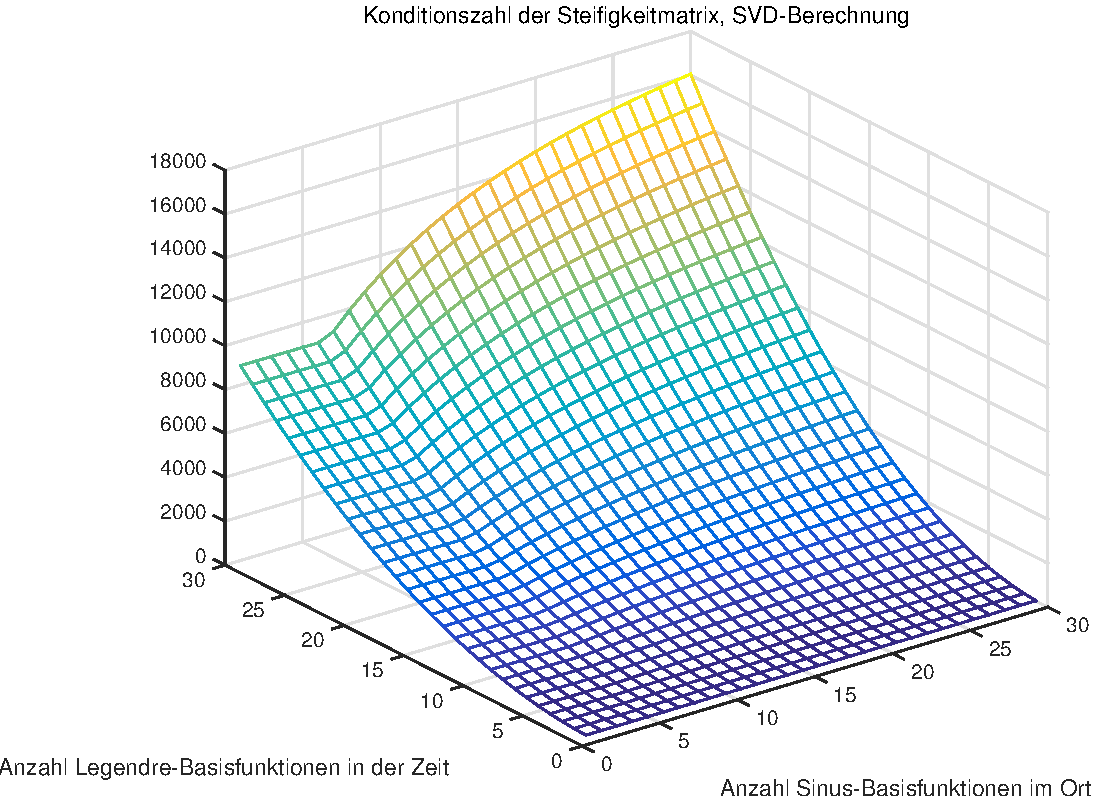
\includegraphics[width=0.9\textwidth]{figures/oned/conds.pdf}
    \end{center}
\end{figure}

\begin{figure}[tb]
    \begin{center}
        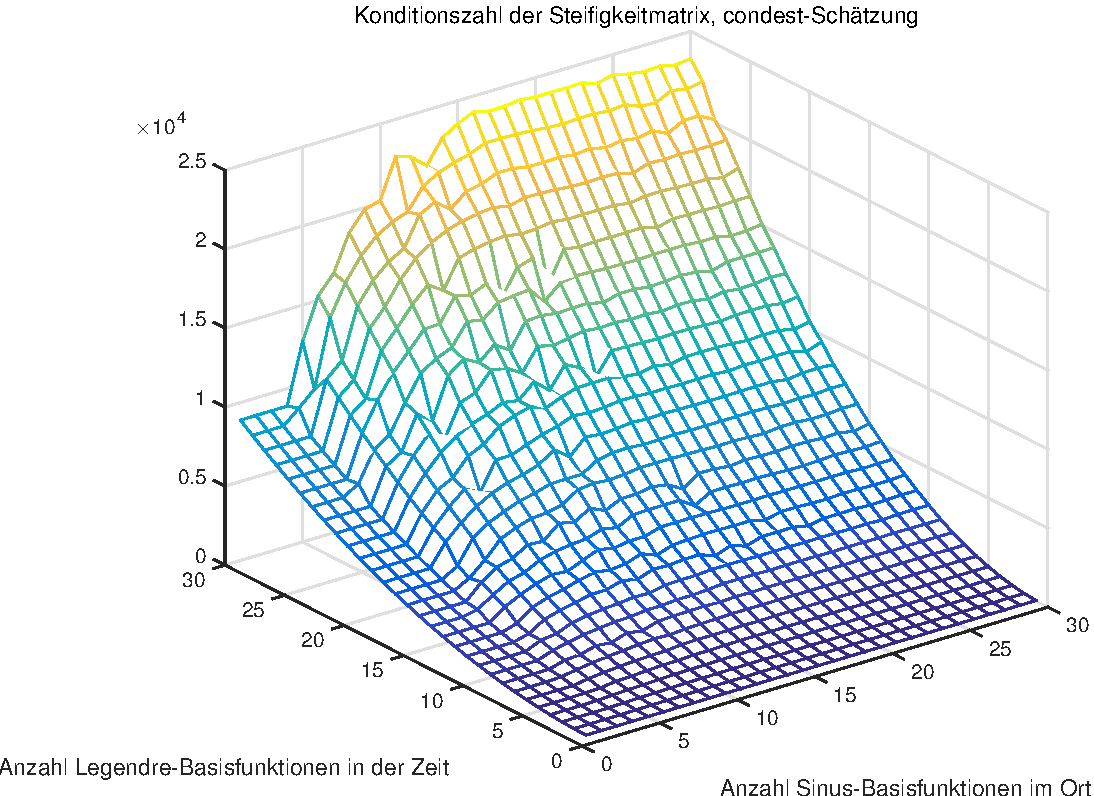
\includegraphics[width=0.9\textwidth]{figures/oned/condest.pdf}
    \end{center}
\end{figure}

\begin{figure}[tb]
    \begin{center}
        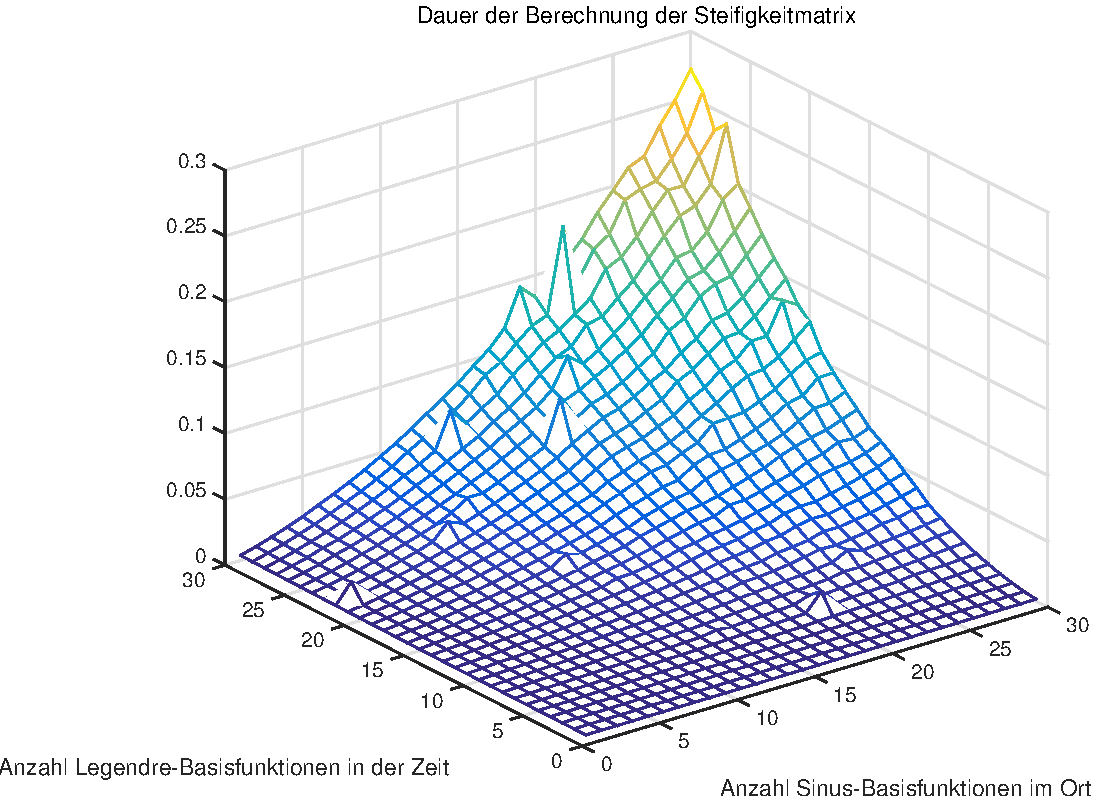
\includegraphics[width=0.9\textwidth]{figures/oned/times.pdf}
    \end{center}
\end{figure}

\begin{figure}[tb]
    \begin{center}
        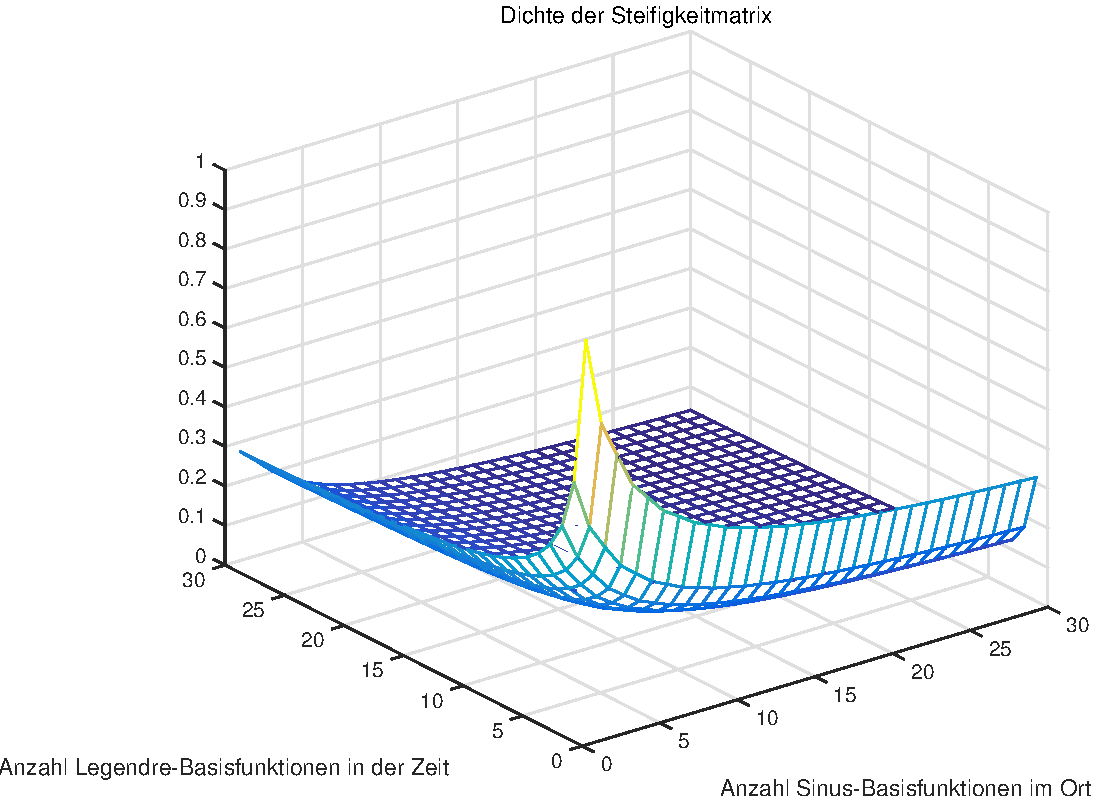
\includegraphics[width=0.9\textwidth]{figures/oned/density.pdf}
    \end{center}
\end{figure}

\clearpage
\begin{landscape}
\thispagestyle{empty}
\begin{table}[tb]
    % \begin{center}
        \hspace{-7em}
        \begin{tabular}{|l|c|c|c|c|c|c|c|c|c|c|c|c|c|c|} \hline
           & 1 & 2 & 3 & 4 & 5 & 6 & 7 & 8 & 9 & 10 & 15 & 20 & 25 & 30 \\  \hline
         1 & 9.09784 & 8.54907 & 7.75467 & 7.69798 & 8.86198 & 10.0584 & 11.1324 & 12.0175 & 12.8546 & 13.5568 & 16.4579 & 18.4241 & 20.2776 & 21.9363 \\ \hline
         2 & 38.2208 & 37.3662 & 35.2039 & 32.6658 & 33.1234 & 37.5904 & 41.4423 & 44.7317 & 47.6463 & 50.2432 & 60.0249 & 66.1611 & 70.1308 & 72.7527 \\ \hline
         3 & 87.5332 &  86.601 & 84.0109 & 80.7416 & 77.0524 & 83.8761 &  92.449 & 99.7869 & 106.263 & 112.055 & 133.772 & 147.373 & 156.093 &  161.84 \\ \hline
         4 & 156.542 & 155.581 &  152.82 & 149.248 & 145.031 & 148.588 & 163.768 & 176.767 & 188.231 &  198.49 &  236.93 & 260.997 & 276.405 & 286.556 \\ \hline
         5 & 245.341 & 244.366 & 241.521 & 237.801 & 233.316 & 231.839 & 255.522 & 275.803 & 293.687 & 309.694 & 369.657 & 407.197 &  431.22 & 447.047 \\ \hline
         6 & 353.892 & 352.909 & 350.018 & 346.215 & 341.578 & 336.131 & 367.678 & 396.861 & 422.594 & 445.626 & 531.902 & 585.913 & 620.473 & 643.239 \\ \hline
         7 & 482.188 & 481.201 & 478.282 & 474.427 & 469.696 & 464.107 & 500.232 & 539.936 & 574.944 &  606.28 & 723.655 & 797.135 & 844.149 &  875.12 \\ \hline
         8 & 630.227 & 629.237 & 626.299 &  622.41 & 617.618 & 611.934 & 653.181 & 705.025 & 750.737 & 791.654 & 944.914 & 1040.86 & 1102.25 & 1142.68 \\ \hline
         9 & 798.007 & 797.014 & 794.063 & 790.152 & 785.316 & 779.568 & 826.525 & 892.128 &  949.97 & 1001.75 & 1195.68 & 1317.08 & 1394.76 & 1445.93 \\ \hline
         10 & 985.526 & 984.533 & 981.572 & 977.644 & 972.778 & 966.982 & 1020.26 & 1101.24 & 1172.64 & 1236.56 & 1475.94 & 1625.81 & 1721.69 & 1784.85 \\ \hline
         15 & 2219.22 & 2218.22 & 2215.24 & 2211.27 & 2206.33 & 2200.42 & 2294.86 & 2477.01 & 2637.61 & 2781.37 & 3319.82 & 3656.89 & 3872.55 & 4014.61 \\ \hline
         20 &  3946.4 &  3945.4 & 3942.41 & 3938.43 & 3933.46 & 3927.51 & 4079.31 & 4403.09 & 4688.57 & 4944.11 & 5901.24 & 6500.43 & 6883.77 &  7136.3 \\ \hline
         25 & 6167.06 & 6166.06 & 6163.07 & 6159.08 &  6154.1 & 6148.13 &  6373.6 & 6879.48 & 7325.51 & 7724.77 & 9220.22 & 10156.4 & 10755.3 & 11149.9 \\ \hline
         30 &  8881.2 &  8880.2 & 8877.21 & 8873.21 & 8868.23 & 8862.25 & 9177.72 & 9906.18 & 10548.4 & 11123.4 & 13276.8 & 14624.8 & 15487.3 & 16055.4 \\ \hline
        \end{tabular}
        \caption{Konditionszahl der Steifigkeitsmatrix $B$. Berechnet anhand der Singulärwerte. Horizontal variiert die Anzahl der Lengdre-Basisfunktionen für die Zeit, vertikal die Anzahl der Sinus-Basisfunktionen für den Raum.}
    % \end{center}
\end{table}
\end{landscape}

\clearpage
\section{Zu klärende Fragen} % (fold)
\label{sec:zu_kl_rende_fragen}

Was?

Konditionszahlen?

% section zu_kl_rende_fragen (end)

% chapter numerische_experimente (end)


    % %!TEX root = ../main.tex

\section{Eindimensionaler Fall mit $\omega \in \mathbb{R}$ und ohne Quellterm}

Sei $I := [0, \hat t]$ für ein $0 < \hat t < \infty$ und $\Omega := [0, 1]$.
Betrachte folgende parametrisierte PDE
\begin{align}
    \begin{cases}
    u_{t}(t, x) = \sigma u_{xx}(t, x) - \omega u(t, x), & (t, x) \in I \times \Omega\\
    u(0, x) = g(x), & x \in \Omega \\
    u(t, 0) = u(t, 1) = 0, & t \in I
    \end{cases}
\end{align}
mit Konstanten $\sigma, \omega \in \mathbb{R}$.

Ein Separation der Variablen Ansatz $u(t, x) = X(x) T(t)$ liefert
\begin{equation}
    X(x)T'(t) = \sigma X''(x) T(t) - \omega X(x) T(t)
\end{equation}
oder auch
\begin{equation}
    \frac{T'(t)}{T(t)} = \sigma \frac{X''(x)}{X(x)} - \omega = \lambda
\end{equation}
mit $\lambda \in \mathbb{R}$.

Ohne Einschränkung sei $\lambda \neq 0$, dann erhalten wir zum einen die Dgl.
    $T'(t) = \lambda T(t)$,
deren Lösung
\begin{equation}
    T(t) = d_{3} e^{\lambda t}
\end{equation}
ist, und zum anderen die Dgl.
    $X''(x) =  \frac{\lambda + \omega}{\sigma} X(x)$
mit der Lösung
\begin{equation}
    X(x) = d_{1} e^{\sqrt{\frac{\lambda + \omega}{\sigma}} x} + d_{2} e^{-\sqrt{\frac{\lambda + \omega}{\sigma}}x},
\end{equation}
wobei $d_{1}, d_{2}, d_{3} \in \mathbb{R}$.

Als nächstes Verwenden wir die Anfangs- und Randbedingungen um die Konstanten $d_{i}$ zu bestimmen.
Sei
\begin{equation}
    u(t, x) = \left( d_{1} e^{\sqrt{\frac{\lambda + \omega}{\sigma}} x} + d_{2} e^{-\sqrt{\frac{\lambda + \omega}{\sigma}}x} \right) \left( d_{3} e^{\lambda t} \right),
\end{equation}
Betrachten wir zunächst die Randbedingung $u(t, 0) = u(t, 1) = 0$, dann erhalten wir aus
\begin{equation}
    0 = u(t, 0) = \left( d_{1} + d_{2} \right) \left( d_{3} e^{\lambda t} \right),
\end{equation}
oder äquivalent $d_{1} = - d_{2}$, und aus
\begin{equation}
    0 = u(t, 1) = \left( d_{1} e^{\sqrt{\frac{\lambda + \omega}{\sigma}}} + d_{2} e^{-\sqrt{\frac{\lambda + \omega}{\sigma}}} \right) \left( d_{3} e^{\lambda t} \right) =
    d_{1} \left( e^{\sqrt{\frac{\lambda + \omega}{\sigma}}} - e^{-\sqrt{\frac{\lambda + \omega}{\sigma}}} \right) \left( d_{3} e^{\lambda t} \right),
\end{equation}
ohne Einschränkung $d_{1} \neq 0$, die Gleichung
\begin{equation}
    0 = e^{\sqrt{\frac{\lambda + \omega}{\sigma}}} - e^{-\sqrt{\frac{\lambda + \omega}{\sigma}}}.
\end{equation}
Aus dieser erhalten wir durch Äquivalenzumformungen
\begin{align}
    e^{\sqrt{\frac{\lambda + \omega}{\sigma}}} - e^{-\sqrt{\frac{\lambda + \omega}{\sigma}}} = 0
    &\quad \iff \quad
    e^{2\sqrt{\frac{\lambda + \omega}{\sigma}}} = 1
    \quad \iff \quad
    \sqrt{\tfrac{\lambda + \omega}{\sigma}} = k \pi i
    \\&\quad \iff \quad
    \tfrac{\lambda + \omega}{\sigma} = -k^2 \pi^2
    \quad \iff \quad
    \lambda = -k^2 \pi^2 \sigma - \omega,
\end{align}
mit $k \in \mathbb{Z}$ beliebig.
Einsetzen liefert nun
\begin{align}
    u_{k}(t, x) &= d_{1} \left( e^{k \pi i x} - e^{-k \pi i x} \right) \left( d_{3} e^{- (k^2 \pi^2 \sigma + \omega) t} \right)
    \\&= 2 d_{1} d_{3} i \sin(k \pi x) e^{-(k^2 \pi^2 \sigma + \omega)t},
\end{align}
wobei wir $\beta_{k} := 2 d_{1} d_{3} i$ setzen.

Da jedes $u_{k}$, $k \in \mathbb{Z}$, eine Lösung ist, erhalten wir durch
\begin{equation}
    u(t, x) = \sum_{k = 1}^{\infty} u_{k}(t, x) = \sum_{k = 1}^{\infty} \beta_{k} \sin(k \pi x) e^{-(k^2 \pi^2 \sigma + \omega)t}
\end{equation}
ebenfalls eine Lösung.
Damit die Anfangsbedingung erfüllt wird, muss
\begin{equation}
    g(x) = u(x, 0) = \sum_{k = 1}^{\infty} \beta_{k} \sin(k \pi x)
\end{equation}
gelten, was genau dann der Fall ist, wenn
\begin{equation}
    \beta_{k} = 2 \int_{0}^{1} g(x) \sin(k \pi x) \diff x.
\end{equation}

Da $u_{k}$ analytisch in $\omega$ für alle $k \in \mathbb{Z}$, ist auch $u$ analytisch in $\omega$ und es gilt
\begin{equation}
    \frac{\partial^{j} u(t, x; \omega)}{\partial \omega^{j}} = \sum_{k = 1}^{\infty} (-t)^{j} \beta_{k} \sin(k \pi x) e^{-(k^{2} \pi^{2} \sigma + \omega)t}.
\end{equation}


    %%%%%%%%%%%%%%%%%%%%%%%%%%%%%%%%%%%%%%%%%%%%%%%%%%%%%%%%%%%%%%%%%%%%%%%%%%%
    %%% Anhang
    \appendix{}
    %!TEX root = ../main.tex

\chapter{Funktionalanalytische Grundlagen} % (fold)
\label{cha:funktionalanalytische_grundlagen}

\section{Orthogonale Funktionen und Polynome}
\label{sec:orthogonale_funktionen_und_polynome}

\begin{Satz}[Orthogonalität trigonometrischer Funktionen]
\label{satz:trigonometrische_funktionen_orthogonal}
    Seien $k, l \in \mathbb{N}$.
    Dann gilt
    \begin{align}
        \skprod{\sin(\pi k x)}{\sin(\pi l x)}_{L_{2}([0, 1])} = \frac{1}{2} \delta_{kl}
        \quad\text{und}\quad
        \skprod{\cos(\pi k x)}{\cos(\pi l x)}_{L_{2}([0, 1])} = \frac{1}{2} \delta_{kl}.
    \end{align}
\end{Satz}

\begin{Definition}[Legendre-Polynome]
\label{definition:legendre_polynome}
    Sei $I = [-1, 1]$.
    Die Legendre-Polynome $L_{n} \in \Pi_{n}$ sind definiert durch
    \begin{equation}
        L_{n}(x) = \frac{1}{2^{n}n!}\frac{\diff^{n}}{\diff x^{n}} (x^{2} - 1)^{n}.
    \end{equation}
    Durch die Transformation $x \mapsto 2x - 1$ erhält man die auf das Interval $[0, 1]$ geshifteten Legendre-Polynome $\tilde L_{n}$.
\end{Definition}

\begin{Satz}[Orthogonalität der Legendre-Polynome]
\label{satz:legendre_polynome_orthogonal}
    Die Legendre-Polynome $L_{n}$ sind orthogonal bezüglich der $L_{2}([-1, 1])$-Norm, denn es gilt
    \begin{equation}
        \skprod{L_{n}}{L_{m}}_{L_{2}([-1, 1])} = \frac{2}{2n + 1} \delta_{n m}.
    \end{equation}
    Auch für die geshifteten Legendre-Polynome $\tilde L_{n}$ gilt Orthogonalität, denn es ist
    \begin{equation}
        \skprod{\tilde L_{n}}{\tilde L_{m}}_{L_{2}([0, 1])} = \frac{1}{2n + 1} \delta_{n m}.
    \end{equation}
\end{Satz}

\begin{Bemerkung}
\label{satz:legendre_polynome_rekursion}
    Die Legendre-Polynome $L_{n}$ erfüllen die Rekursionsformel
    \begin{equation}
        n L_{n}(x) = (2n - 1) x L_{n-1}(x) - (n - 1) L_{n-2}(x), \quad L_{0}(x) = 1, L_{1}(x) = x.
    \end{equation}
    Analog gilt für die erste Ableitung $L_{n}'$ die Rekursionsformel
    \begin{equation}
        (n - 1) L_{n}'(x) = (2n -1) x L_{n-1}'(x) - n L_{n-2}'(x), \quad L_{0}'(x) = 0, L_{1}'(x) = 1.
    \end{equation}
\end{Bemerkung}

\section{Sonstiges} % (fold)
\label{sec:sonstiges}

% \begin{Lemma}
%     $\mathcal C^{0}([a, b]; X)$ liegt dicht in $L_{p}(a, b; X)$ für $1 \leq p < \infty$.
% \end{Lemma}

\begin{Satz}[Poincaré-Friedrichs-Ungleichung, vgl. {{\cite[Theorem II.1.7]{Braess:2007wm}}}]
\label{satz:grundlagen:poincare_friedrichs_ungleichung}
    Es sei $\Omega \subset \mathbb{R}^{n}$ beschränkt und in einem $n$-dimensionalen Würfel mit Seitenlänge $s$ enthalten.
    Dann gilt
    \begin{equation}
        \label{eq:grundlagen:poincare_friedrichs_ungleichung}
        \abs{u}_{H^{m}} \leq \norm{u}_{H^{m}} \leq (1 + s)^{m} \abs{u}_{H^{m}} \quad \text{für alle}~u \in H^{m}_{0}(\Omega).
    \end{equation}
\end{Satz}

\begin{Lemma}[vgl {{\cite[Remark 2.1.48]{Sauter:9_WoPZ0Y}}}]
\label{lemma:sauter:2.1.48}
    Seien $X$ und $Y$ zwei reflexive Banachräume und $a \colon X \times Y \to \mathbb{R}$ eine Bilinearform.
    Finden wir für jedes $x \in X$ ein $y_{x} \in Y$, so dass
    \begin{equation}
        \label{eq:lemma:sauter:2.1.48:eq1}
        \abs{a(x, y_{x})} \geq C_{1} \norm{x}_{X}^{2} \quad \text{und} \quad \norm{y_{x}}_{Y} \leq C_{2} \norm{x}_{X}
    \end{equation}
    mit von $x$ und $y_{x}$ unabhängigen Konstanten $C_{1}, C_{2} > 0$ gilt, dann folgt daraus die inf-sup-Bedingung
    \begin{equation}
    \label{eq:lemma:sauter:2.1.48:inf_sup}
        \inf_{0 \neq x \in X} \sup_{0 \neq y \in Y} \frac{a(x, y)}{\norm{x}_{X}\norm{y}_{Y}} \geq \gamma > 0
    \end{equation}
    mit $\gamma = \frac{C_{1}}{C_{2}}$.

    \begin{Beweis}
        Seien $x \in X$ und $y_{x} \in Y$ so, dass \eqref{eq:lemma:sauter:2.1.48:eq1} erfüllt ist.
        Dann gilt
        \begin{align}
            \inf_{0 \neq x \in X} \sup_{0 \neq y \in Y} \frac{\abs{a(x, y)}}{\norm{x}_{X} \norm{y}_{Y}}
            &\geq
            \inf_{0 \neq x \in X} \frac{\abs{a(x, y_{x})}}{\norm{x}_{X} \norm{y_{x}}_{Y}}
            \\&\geq
            \inf_{0 \neq x \in X} \frac{C_{1} \norm{x}^{2}_{X}}{\norm{x}_{X} C_{2} \norm{x}_{X}}
            =
            \frac{C_{1}}{C_{2}}
            > 0.
        \end{align}
    \end{Beweis}
\end{Lemma}

% section sonstiges (end)


    % Abbildungs-, Tabellen- und Symbolverzeichnis
    % \listtheorems
    % \listoffigures
    % \listoftables
    \printnomenclature

    % Literaturverzeichnis
    \printbibliography

    % Anhänge

    % Eidesstattliche Erklärung
    % %!TEX root = ../main.tex

\chapter{Eidesstattliche Erklärung} % (fold)
\label{cha:eidesstattliche_erklaerung}

Ich versichere hiermit, dass ich die vorliegende Masterarbeit selbständig
verfasst und keine anderen als die angegebenen Quellen und Hilfsmittel benutzt
habe, wobei ich alle wörtlichen und sinngemäßen Zitate als solche gekennzeichnet
habe. Die Arbeit wurde bisher keiner anderen Prüfungsbehörde vorgelegt und auch
nicht veröffentlicht.\\[6ex]

\ort, den \today

\hdashrule[-0.5cm]{5cm}{0.5pt}{1pt}

\textsc{\autor}

% chapter eidesstattliche_erklaerung (end)

\end{document}
